\subsection{Overview}
For version 1 onward, we decided to host our website on Amazon Mechanical Turk (AMT), which is a crowd-sourcing website that hosts different machine learning annotation taskss. In the remaining text, we use the word \textit{turker} to refer to annotators that we recruit on AMT; we will also use the word \textit{HIT}, Human Intelligence Task, to refer to a task hosted on AMT. Please refer to \href{https://www.mturk.com/worker/help#:~:text=A%20Human%20Intelligence%20Task%2C%20or,be%20completed%20by%20Worker%20customers.}{AMT FAQs} for official definition and answers to questions related to AMT. 
 
We have to design the following sections for the task: 
\begin{enumerate}
    \item \label{v1_sec_1} an interface containing the main task
    \item instructions and requirements to describe the tasks and specify what the annotators should and should not include in the annotations
    \item a qualification task accompanying the main task to train the turkers to produce high-quality annotations
\end{enumerate}
Compared to Version 0, which we only dabbled with \ref{v1_sec_1} in the above list, we went through all three stages for Version 1 and eventually deployed a pilot.
After deployment, we realized that a few major problems from this design: (1) due to the subjective nature of drawing, it was hard to understand in what ways some annotators are illustrating the given prompts, thus making it difficult to determine the quality of the annotations; (2) turkers are taking more than 30 minutes for each task, showing that providing both sketches and descriptions are inefficient; (3) some turkers are unable to provide descriptions that align with the objects they meant to annotate for; for example, in one step, they drew both eyes and hair, but they only annotate ``big eyes''.      

% Version 1 was the first version to be deployed 
% another version that we did not use as the final interface for data collection. 
% However, compared to version 0, we (1)

\subsection{Interface Design}

\subsubsection{Main Task}
Compare to version 0, we make the following changes to the task interface: 
\begin{enumerate}
    \item Since turkers are paid based on time spent on the task, we decided to forsake the functionality related to the recording and replaying the drawing board.
    \item Since we decide to not limit the drawings to be compositions of basic geometric objects, we removed the step to select primitive shape preceding drawing each component.
\end{enumerate}

\begin{figure*}[!htb]
\begin{subfigure}{\textwidth}
    \centering
    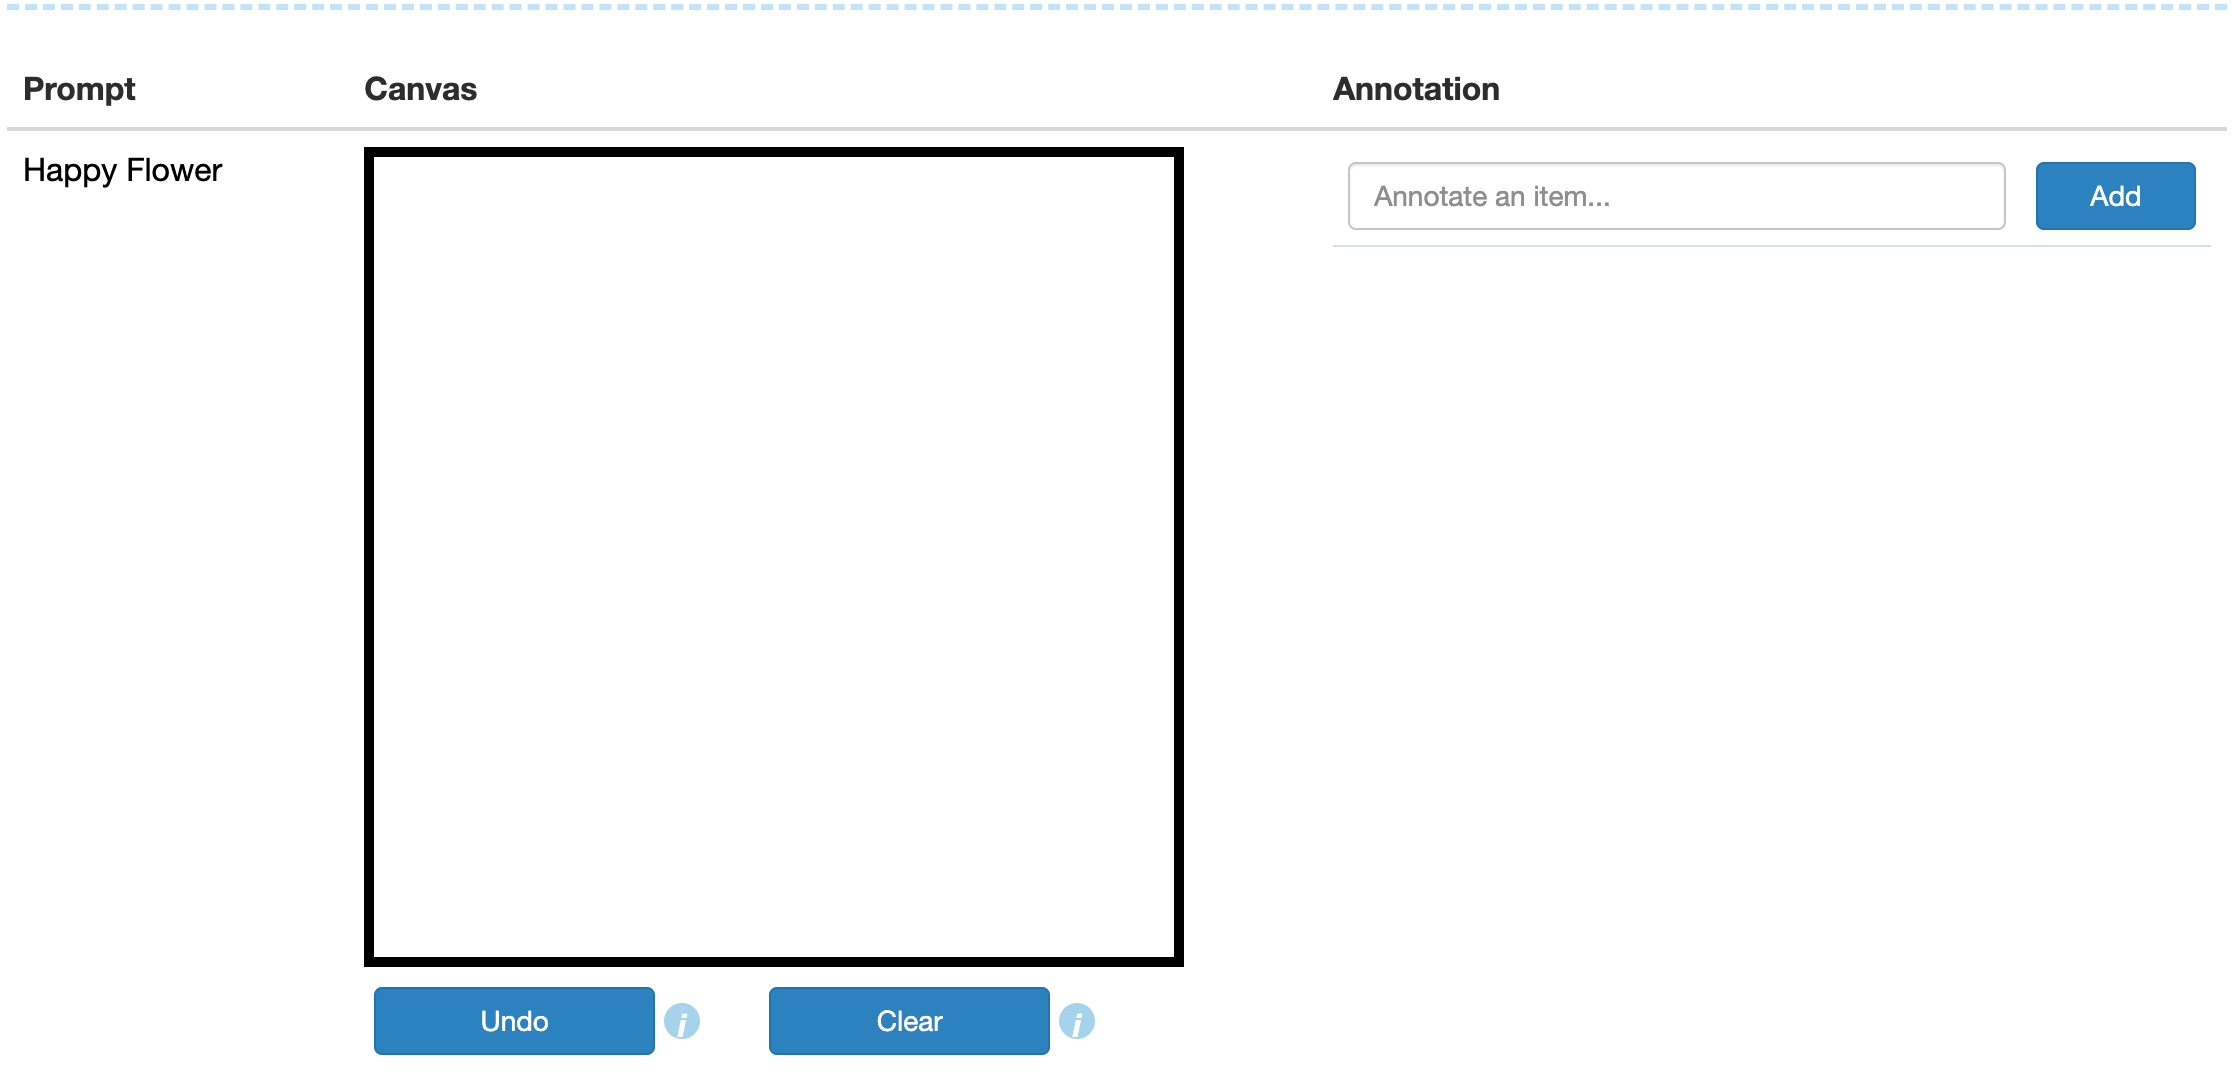
\includegraphics[width=.8\linewidth]{data_collection/v1_empty_table.png}  
    \caption{Main task interface at the start of annotation.}
    \label{v1.main_task.1.a}
\end{subfigure}
\newline
\begin{subfigure}{\textwidth}
    \centering
    % include third image
    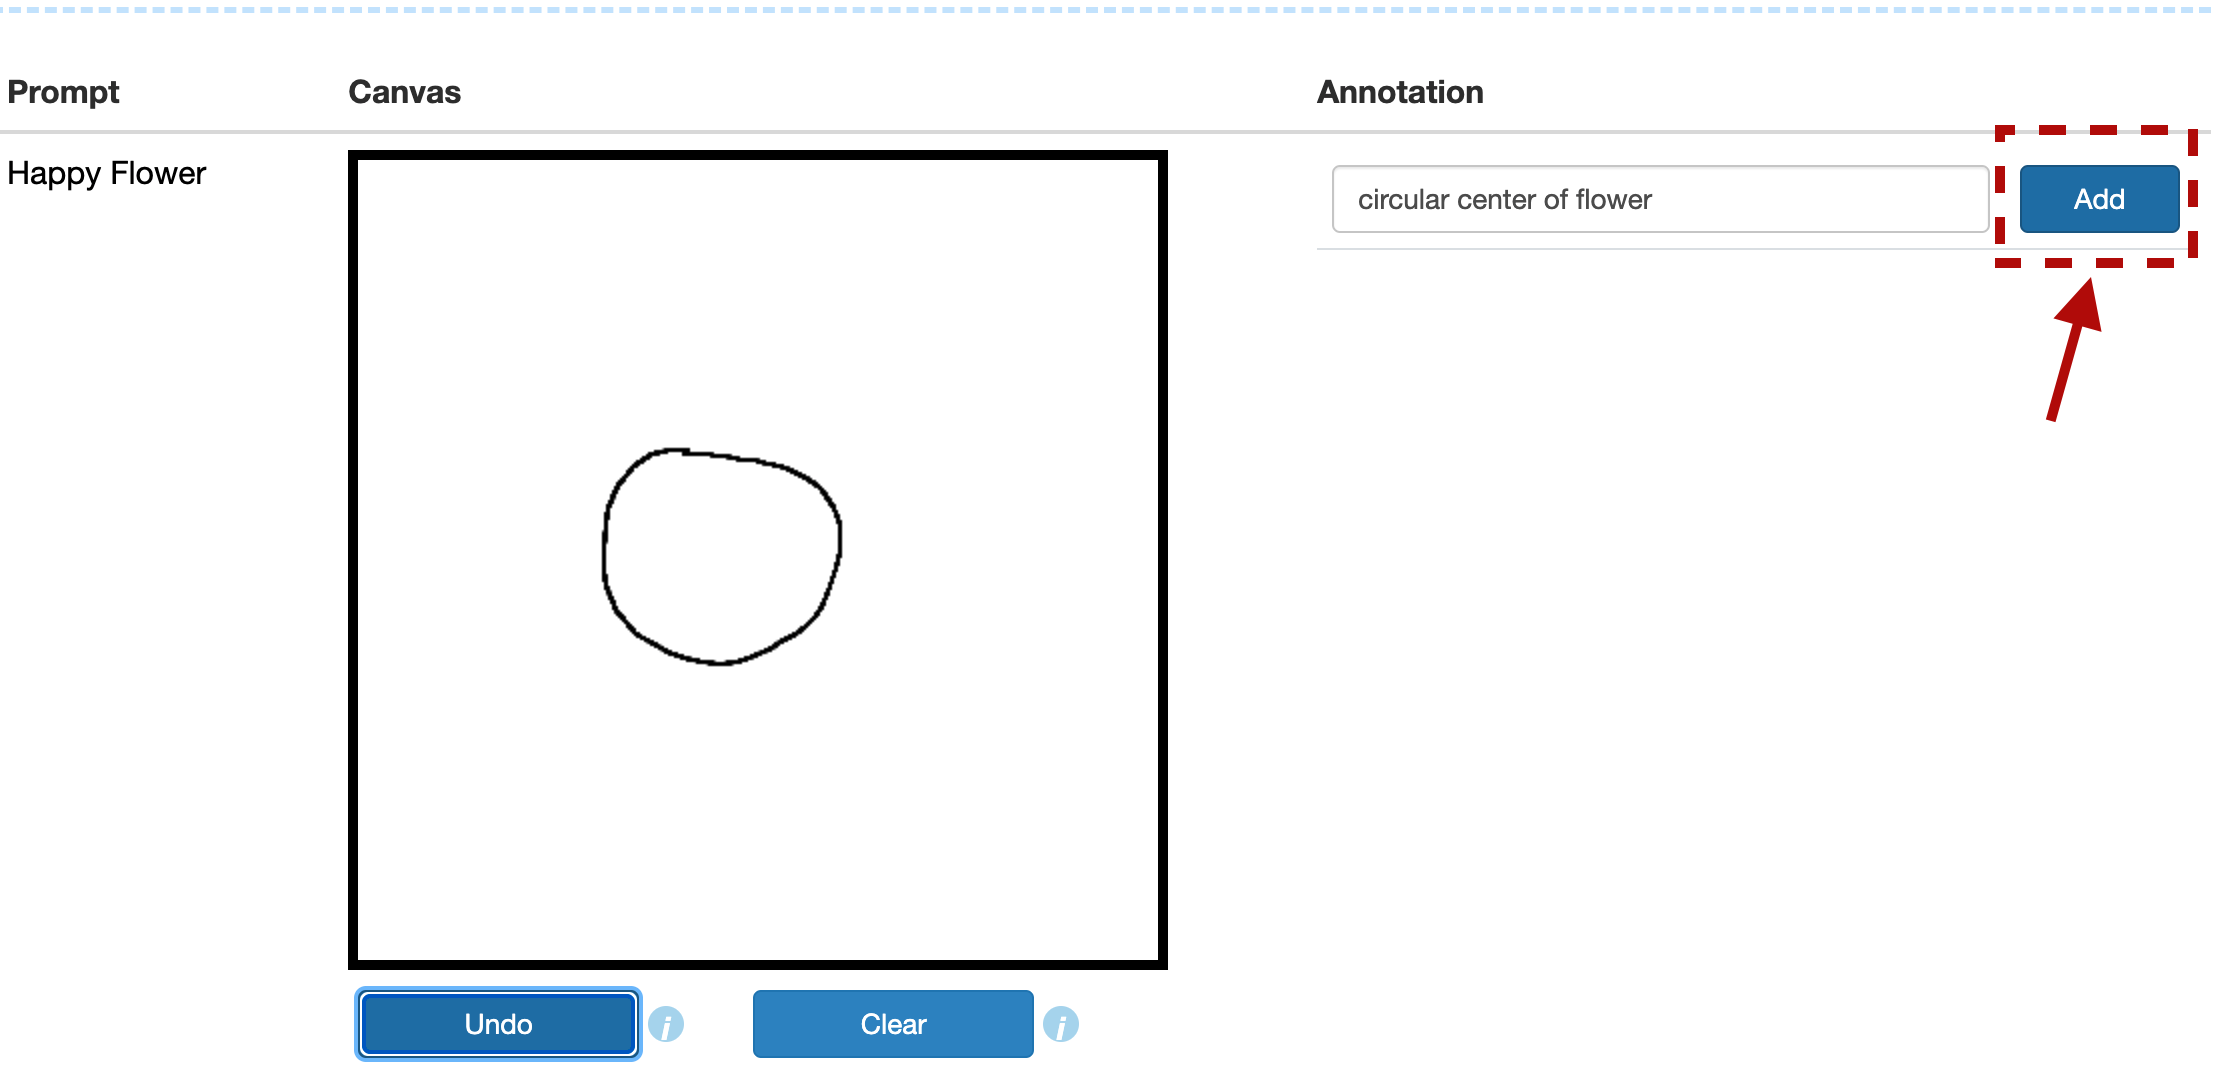
\includegraphics[width=.8\linewidth]{data_collection/v1_before_enter_text.png}  
    \caption{Main task interface before adding text descriptions for the drawing in the given step. Red arrow and box show where to click to add the text.}
    \label{v1.main_task.1.b}
\end{subfigure}
\end{figure*}

\begin{figure*}[!htb]
\ContinuedFloat
\begin{subfigure}{\textwidth}
    \centering
    % include third image
    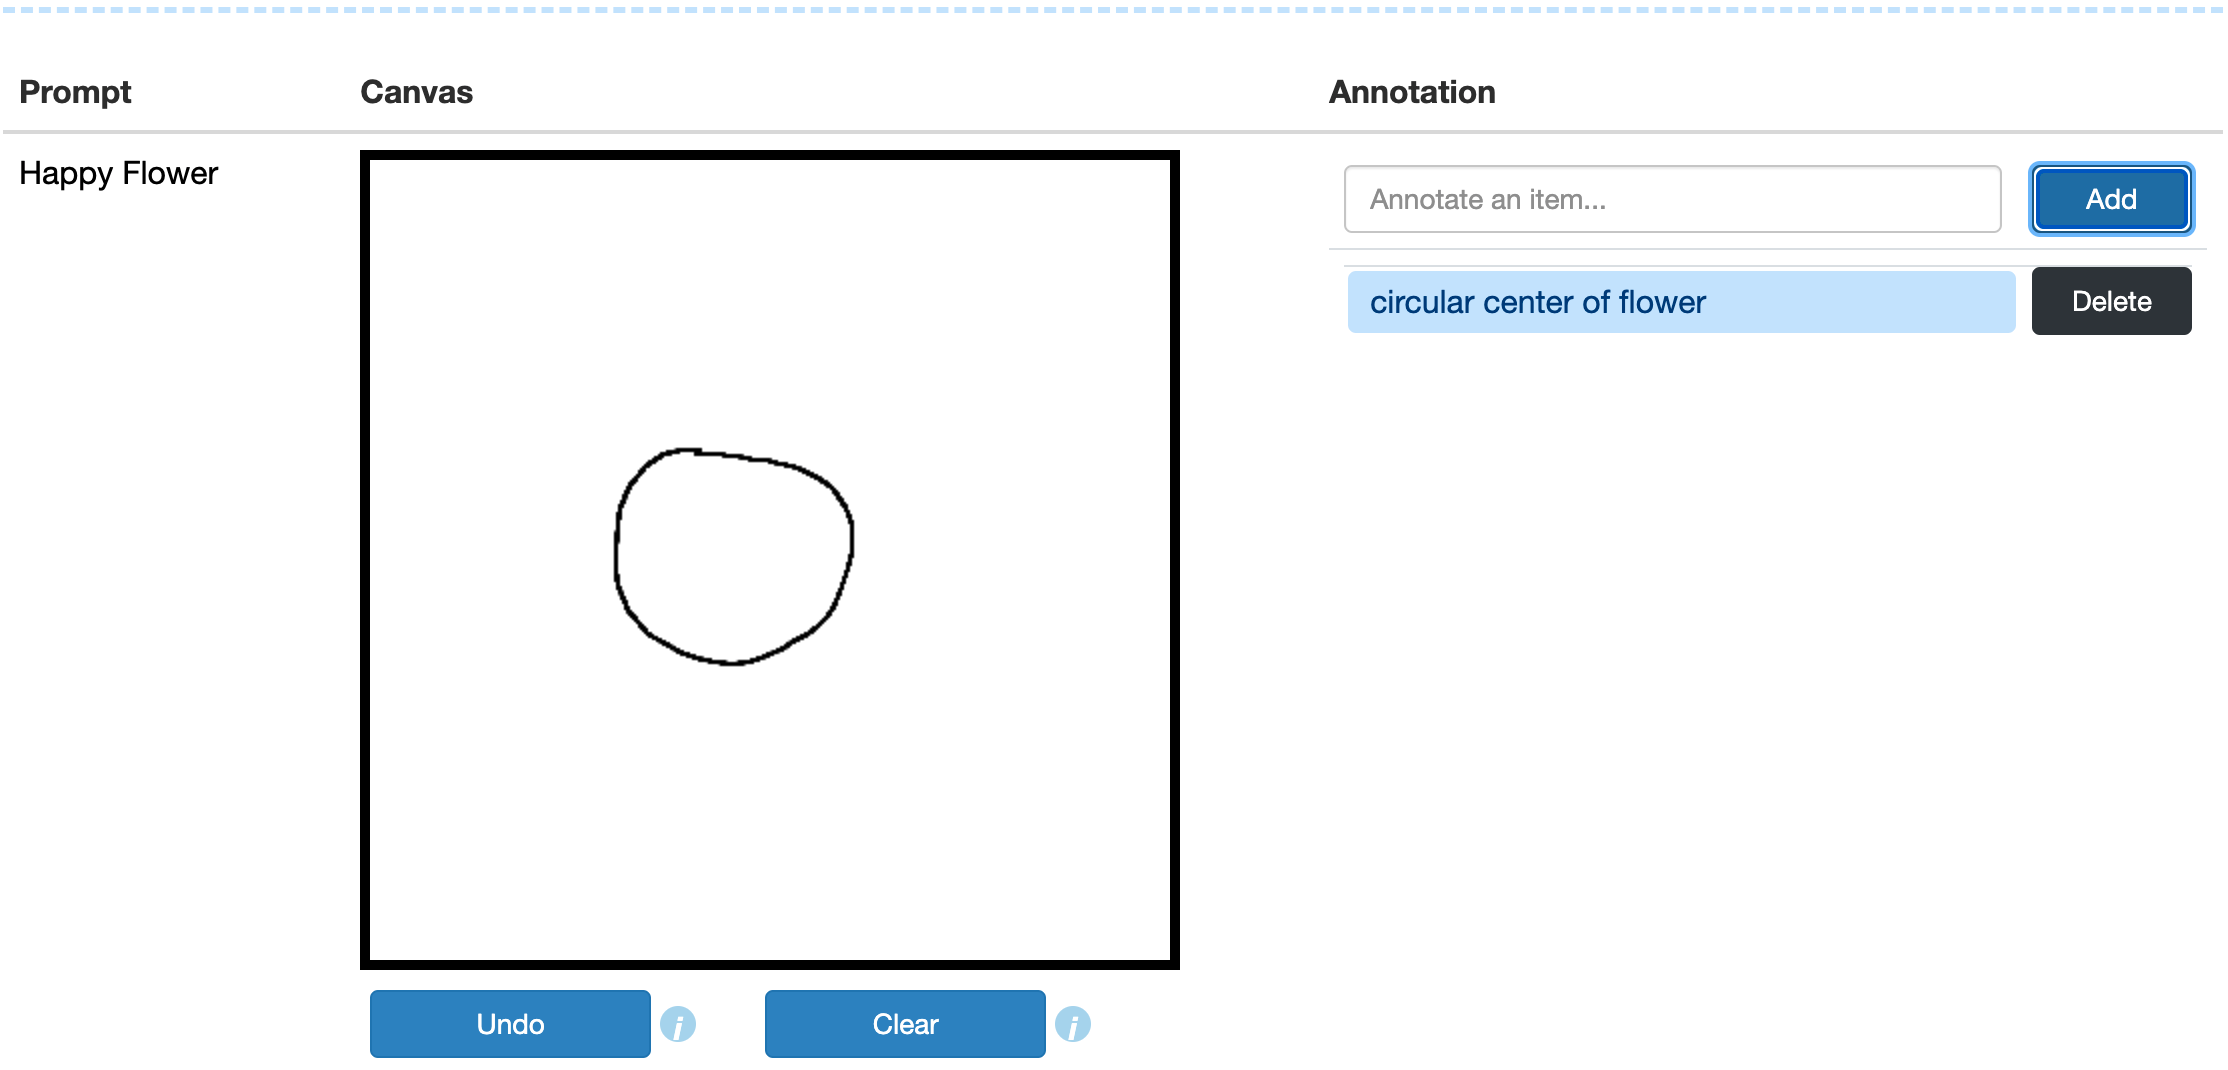
\includegraphics[width=.8\linewidth]{data_collection/v1_after_enter_text.png}  
    \caption{Main task interface after adding text descriptions for the drawing in the given step.}
    \label{v1.main_task.1.c}
\end{subfigure}
\caption{The ``drawing-and-adding'' functionality in Version 1. Repeat the above process for each step in a sketch.}
\label{v1.main_task.1}
\end{figure*}

We illustrate a typical annotation process with Version 1's interface in Figure \ref{v1.main_task.1}. 
The annotator starts with an empty canvas and empty table for textual descriptions, as shown in Figure \ref{v1.main_task.1.a}. For the annotator's convenience, we include a \textit{Undo} button and a \textit{Clear} button for erasing strokes and clearing the entire canvas.  
Then, the annotator draws a step in the sketch, and they would need to enter the text description for this step into the \textit{Annotation} column and hit \textit{Add} to display it as a new row in the annotation table. (Figure \ref{v1.main_task.1.b} and \ref{v1.main_task.1.c} show what the annotation table looks like before and after adding the texts for a given step.) If the annotator wants to remove an entire step, the objects in the drawing and the text description, they can use the \textit{Delete} button next to the texts to do so. An example is shown in Figure \ref{v1.main_task.delete}.
Repeat the drawing-and-adding process until the drawing is done. 
The design of a table for adding and deleting text annotations intends to encourage turkers to break their drawing into a series of semantically meaningful parts, responding to principal \ref{data_design_2} and \ref{data_design_3}.  Enabling users to be able to delete each component is also demonstrative of these two principals. 


\begin{figure*}[!htb]
\begin{subfigure}{\textwidth}
    \centering
    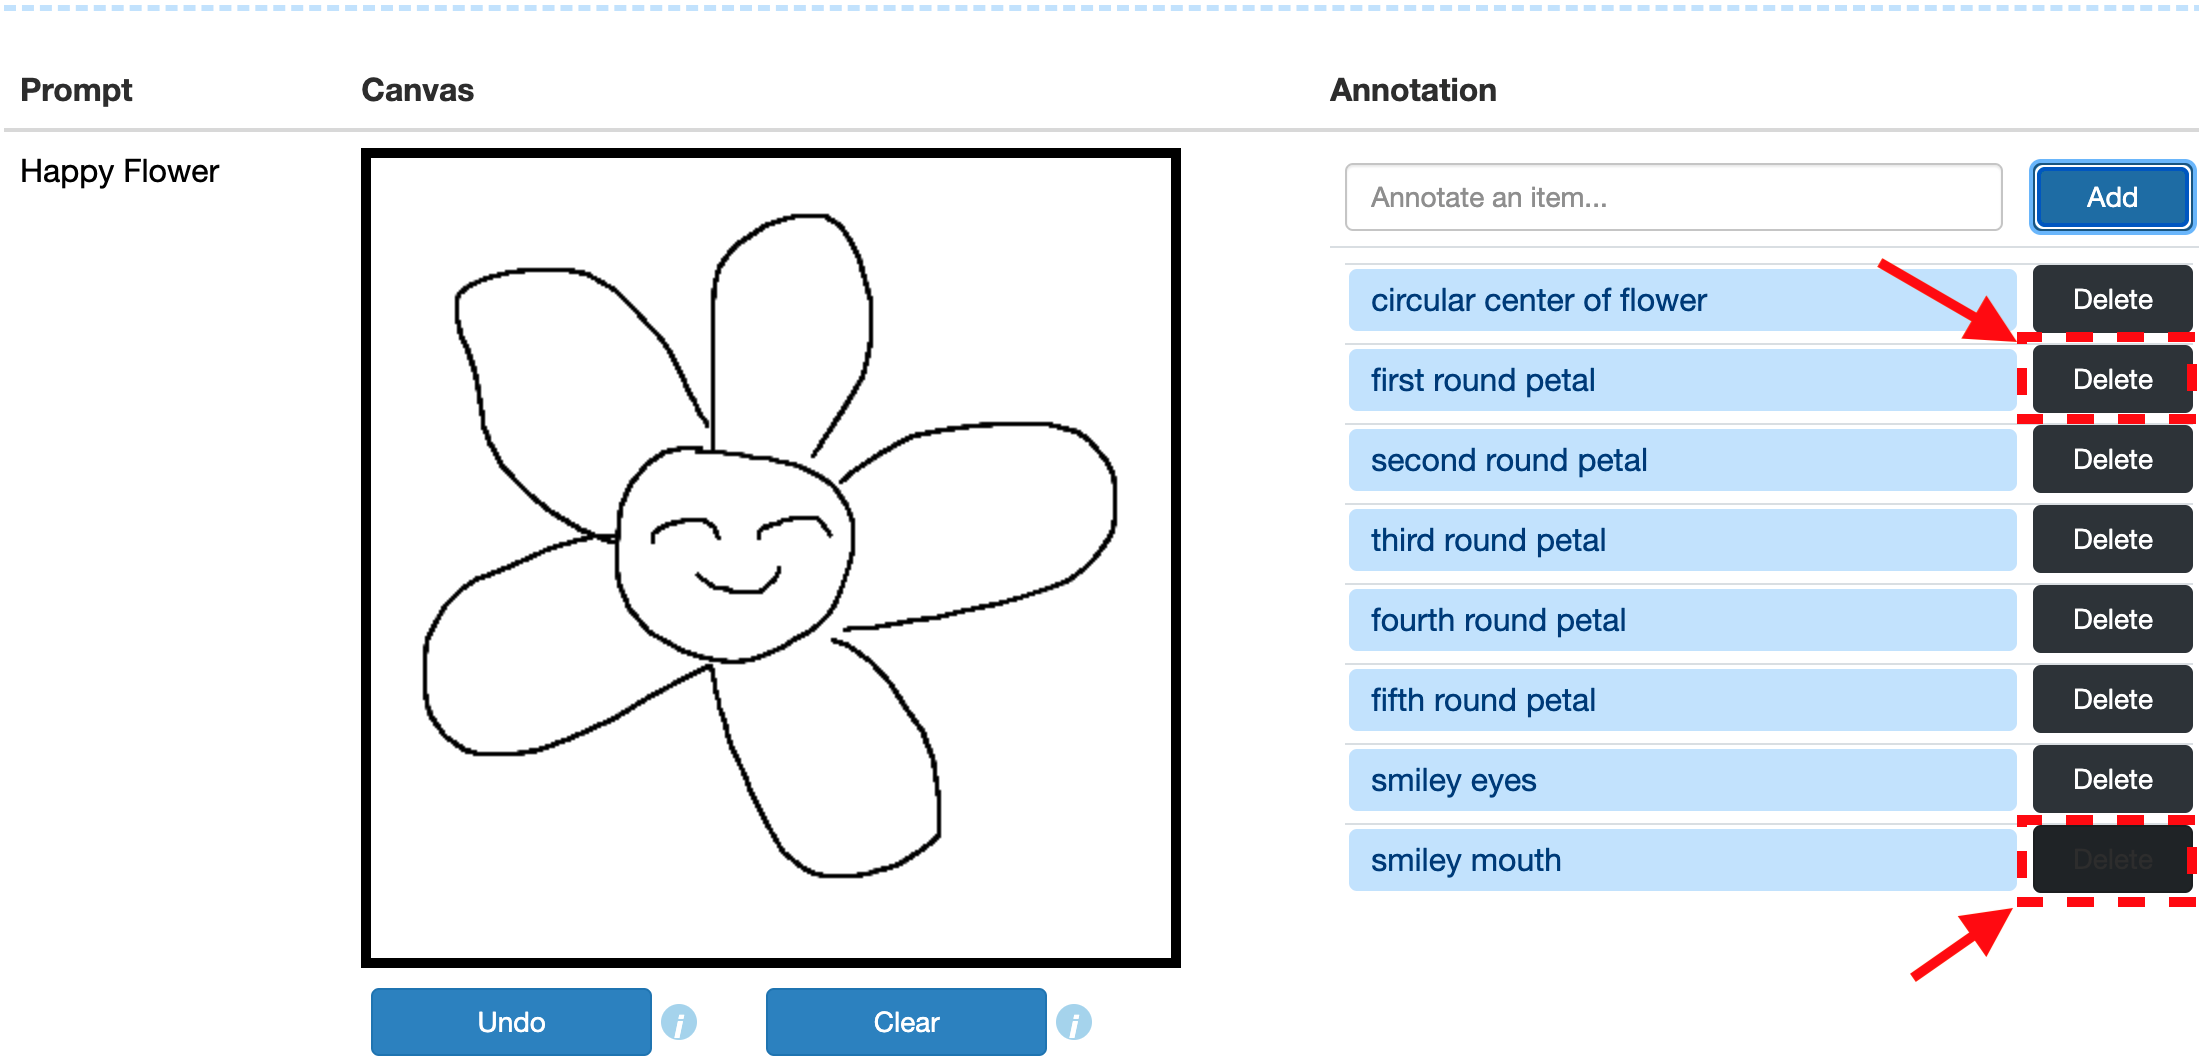
\includegraphics[width=.8\linewidth]{data_collection/v1_before_delete.png}  
    \caption{A complete annotation for the prompt \textit{Happy Flower}. Red arrows and boxes point to \textit{Delete} buttons that can be used to delete the steps associated with the textual annotaitons, if the annotator is not satisfied with the steps.}
    \label{v1.main_task.delete.a}
\end{subfigure}
\newline
\begin{subfigure}{\textwidth}
    \centering
    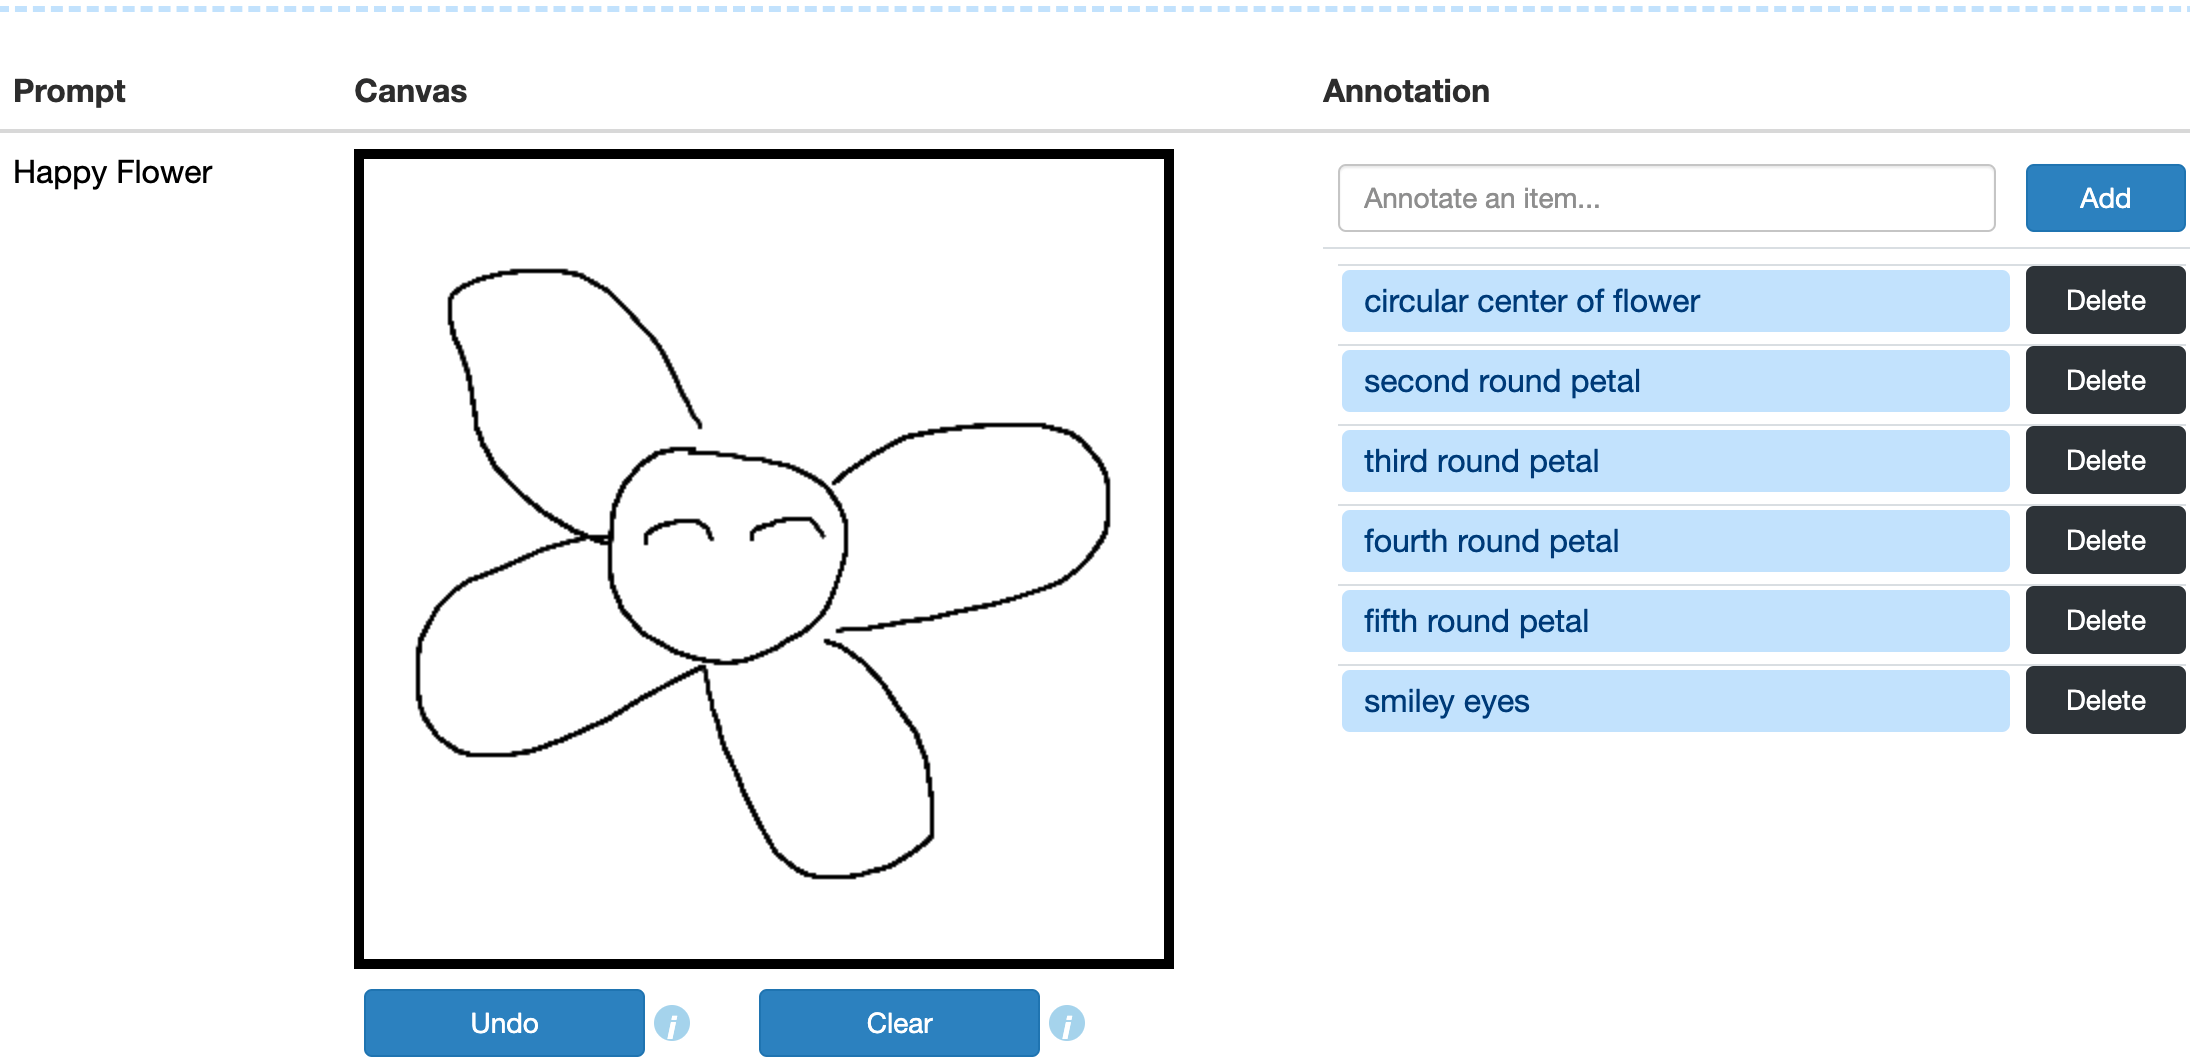
\includegraphics[width=.8\linewidth]{data_collection/v1_after_delete.png}  
    \caption{Main task interface after the two steps associated with \textit{first round petal} and \textit{smiley mouth}, respectively.}
    \label{v1.main_task.delete.b}
\end{subfigure}
\caption{Demonstrating the functionality of the \textit{Delete} button.}
\label{v1.main_task.delete}
\end{figure*}

We encountered some difficulties when implementing the \textit{Delete} functionality. At the beginning, we treated erasing strokes as drawing the same strokes but in white color; however, when strokes overlap each other, overwriting with white strokes would break other strokes into segments. Therefore, we designed the drawing canvas to use layers like Photoshop, so that deleting strokes would be the same as deleting an entire layer, thus leaving other strokes intact.   

\subsubsection{Instruction and Requirement}

\begin{figure*}[!htb]    
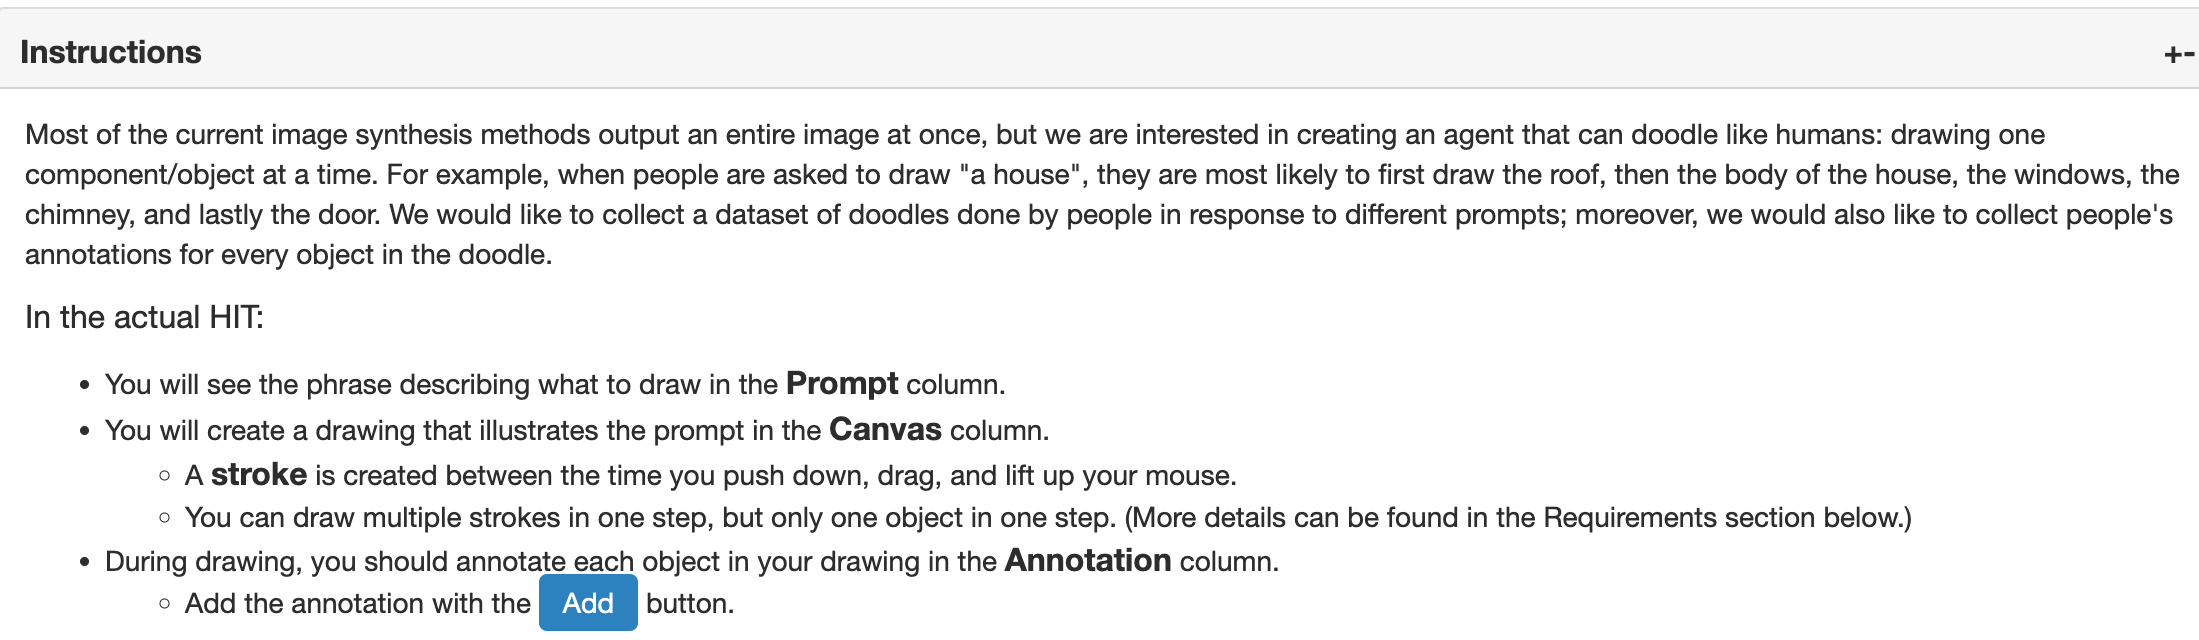
\includegraphics[width=\linewidth]{data_collection/v1_instruction.png} 
\caption{Instruction section of Version 1.}
\label{v1.instruction}
\end{figure*}

We show the layout of the instructions in Figure \ref{v1.instruction}. We begin the instruction by giving a short explantion on the motivation behind collecting this dataset to prime turkers for good-quality annotations, since they would understand more about what the purpose for collecting this dataset. What we struggled the most when drafting the requirements was deciding what would be a single \textit{step} in drawing and how do we clearly explain this definition to the turkers? In Version 0, we relied on common geometric shapes to decompose a drawing into a sequence of steps. In Version 1, we considered asking turkers to annotate for each stroke in the drawing, but we quickly ruled out this option since it was time-consuming, and it did not align with how the instructor taught the child in the \textit{How To Draw a Cute Ice-Cream Cone} video. We decided that turkers should annotate for each \textit{object} in the drawing. The ambiguity around the word \textit{object} has posed the biggest challenge in defining a clear set of requirements. For example, when drawing for the prompt \textit{Happy Face}, one reasonable decomposition is annotating for 4 steps: face, eyes, mouth, and the face contour. However, for someone who draws very detailed eyes, they might want to annotate for the shape of the eye socket and the length of the eye lashes. So what level of specificity should be allowed?  
There is a wide spectrum of allowed annotations depending on how a person approaches drawing for the give prompt. Indeed, the great variation and uncertainty that comes from individuality and personal styles demonstrated through drawings would eventually drive us to not collect drawings and simply ask for text annotations for sketches found in existing datasets.  
At the time, we resorted to repeatedly testing the interface with lab mates to refine the requirements. Here is an excerpt from an old version of the instructions, in which we tried to explain a single \textit{step} of the annotation:
\begin{quotation}
In each task, we show \textbf{1 prompt} from which we would like to get
\begin{enumerate}
    \item A drawing containing 1 \textbf{entity} that you think illustrates the prompt.
    \item Text annotation for every \textbf{``component''} that makes up the entity.
    The word ``component'' is intentially vague, and it depends on how you compose your drawing. For example, in the above example, the prompt is ``smiley face'', and during the process of creating a ``smiley face'' entity, we used 4 components: a face, a left eye, a right eye, and a mouth. For each component, you can annotate with ``face'', ``left eye'', ``right eye'', ``mouth'', respectively; you can also annotate with more details describing the shapes of each component: ``face that looks like an arc opening downwards'', ``a left eye that is an arc'', ``a right eye that looks exactly like the left eye'', ``an arc-like mouth''. Try to use creative and descriptive languages. You can draw a component using multiple strokes.
\end{enumerate}
\end{quotation}
We also need to come up with examples explaining each requirement. We select a few major sub-versions of the requirements resulted from circulating the interface within our lab.  

Requirements and selected examples used in the first release in lab (Item 1 to 3 meant to enforce principal \ref{data_design_1}; Item 4 to 6 for \ref{data_design_2} and \ref{data_design_3}):
\begin{enumerate}
\item Do not draw entity that does not respond to the prompt. For example, given the prompt \textit{Smiley Face}, the drawing should not contain irrelevant objects like a house. 
\item Do not draw more than one entity that responds to the prompt. For example, One should not draw two \textit{Smiley Face} entities, although each \textit{Smiley Face} entity is good. However, you can draw multiple tree objects to illustarte the prompt \textit{Forest}.  
\item \label{v1_requirement1_3} Do not draw entity that is ambiguous in terms of illustrating the prompt. For example, the drawing (Figure \ref{v1.requirement_1.1}) looks more like a \textit{Sad Face} than \textit{Smiley Face}.
\item Do not draw one component that contains more information/content than what the annotation for that component describes. (A counterexample is illustrated in Figure \ref{v1.requirement_1.2}.)
\item Do not split the drawing of a component into multiple steps, unless you can annotate each step separately. (A counterexample is illustrated in Figure \ref{v1.requirement_1.3}.)
\item Do not annotate a component more than once.
\end{enumerate}

\begin{figure*}[!htb]
\begin{subfigure}{0.5\textwidth}
    \centering
    
\includegraphics[width=.4\linewidth]{data_collection/host_amazon/hit_1/bad_smiley_face_ambiguous_face.png}  
    \caption{An example included in the first version of the requirements, explained in more details in item \ref{v1_requirement1_3}.}
    \label{v1.requirement_1.1}
\end{subfigure}
\end{figure*}

\begin{figure*}[!htb]
\ContinuedFloat
\begin{subfigure}{\textwidth}
    \centering
    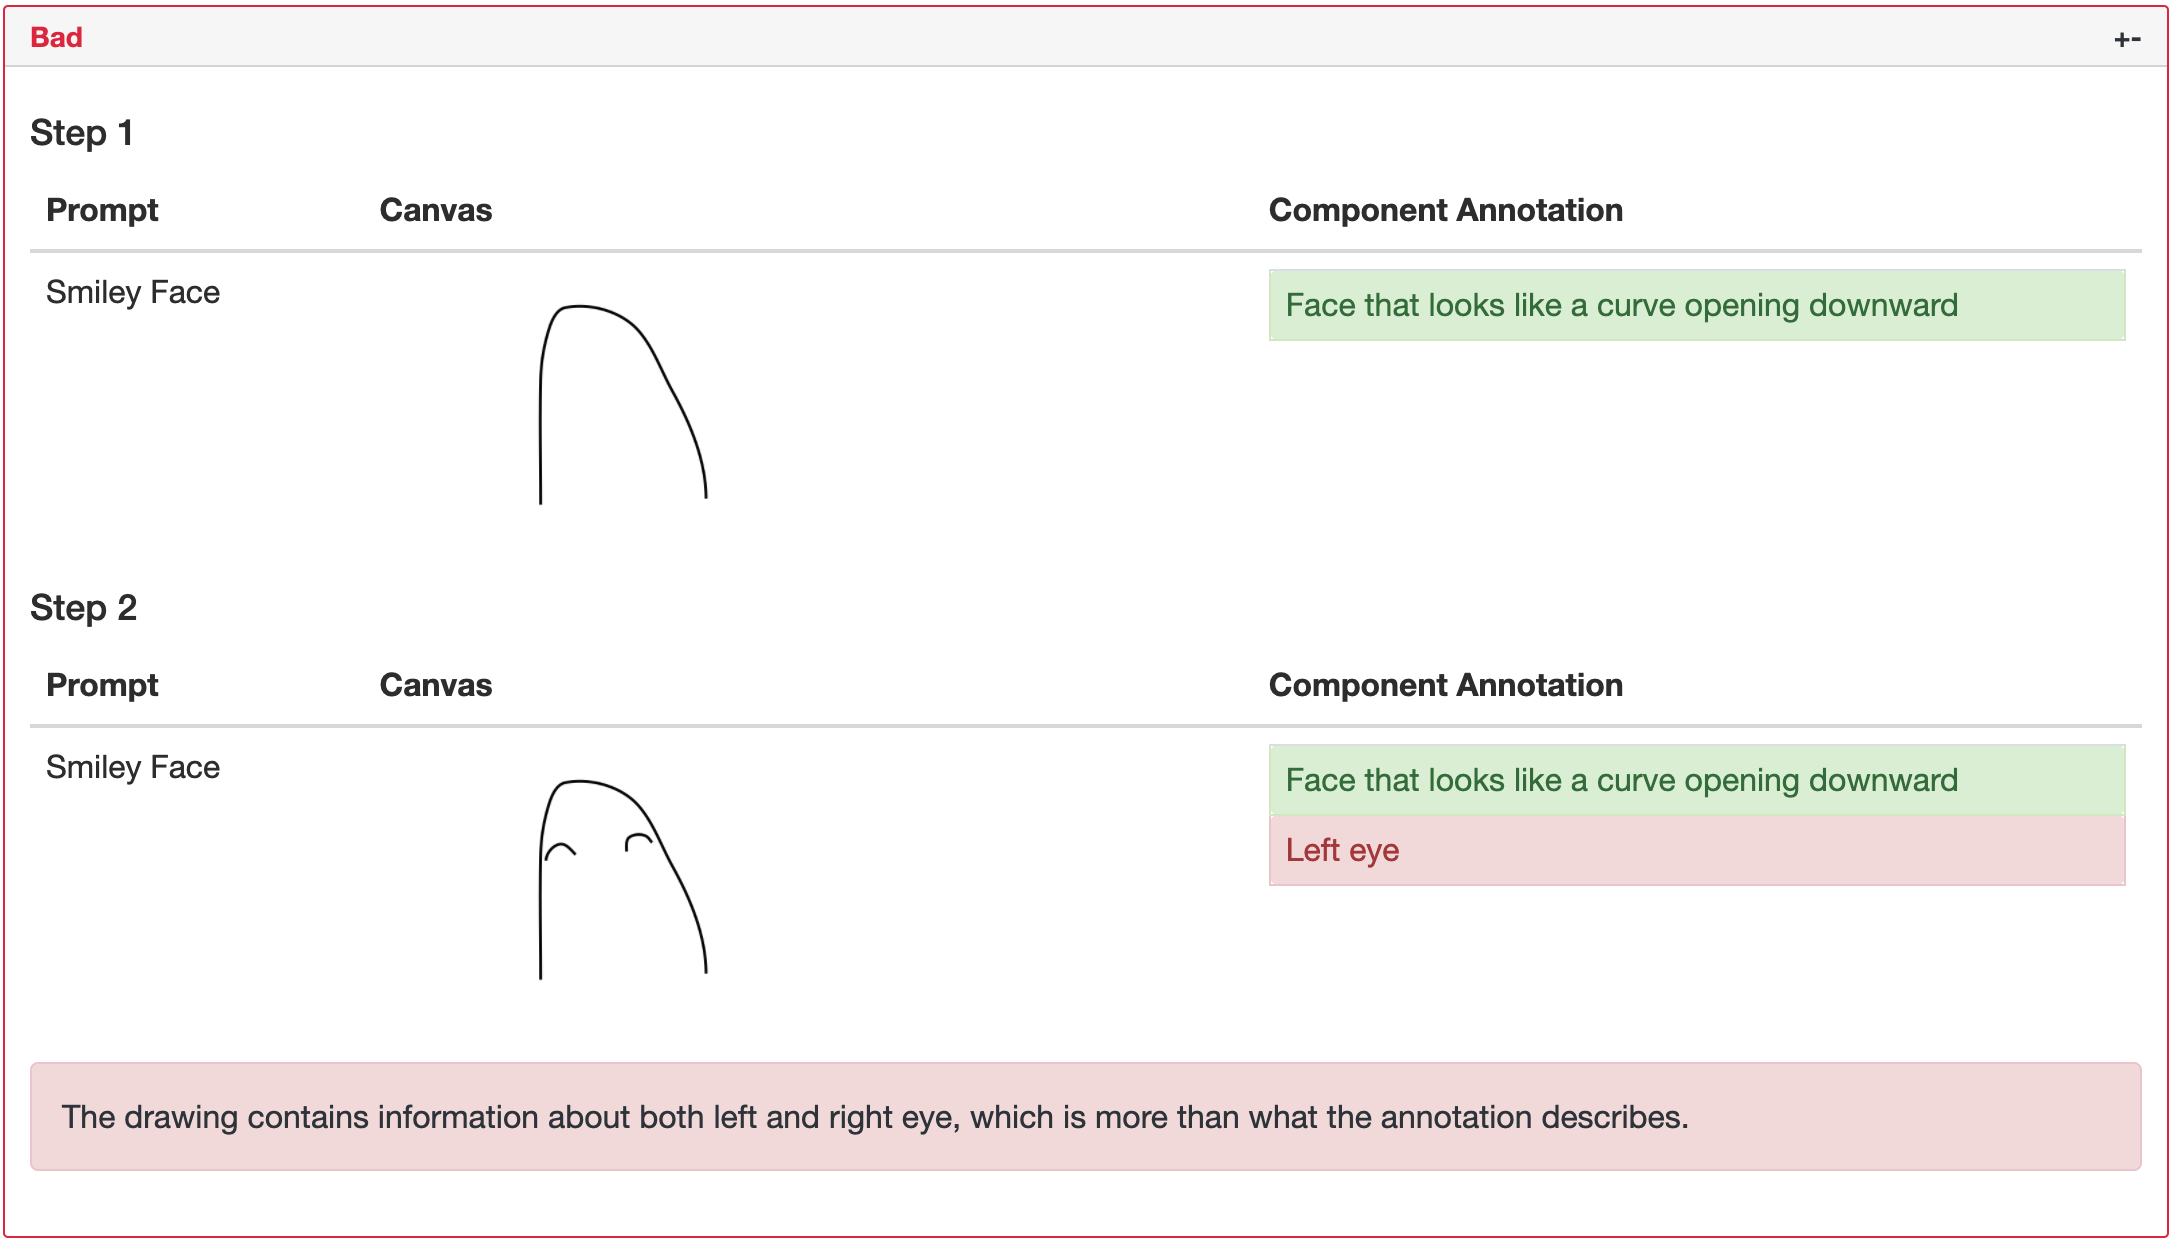
\includegraphics[width=.8\linewidth]{data_collection/v1_requirement1_bad1.png}  
    \caption{Unaligned drawing and text description.}
    \label{v1.requirement_1.2}
\end{subfigure}
\newline
\begin{subfigure}{\textwidth}
    \centering
    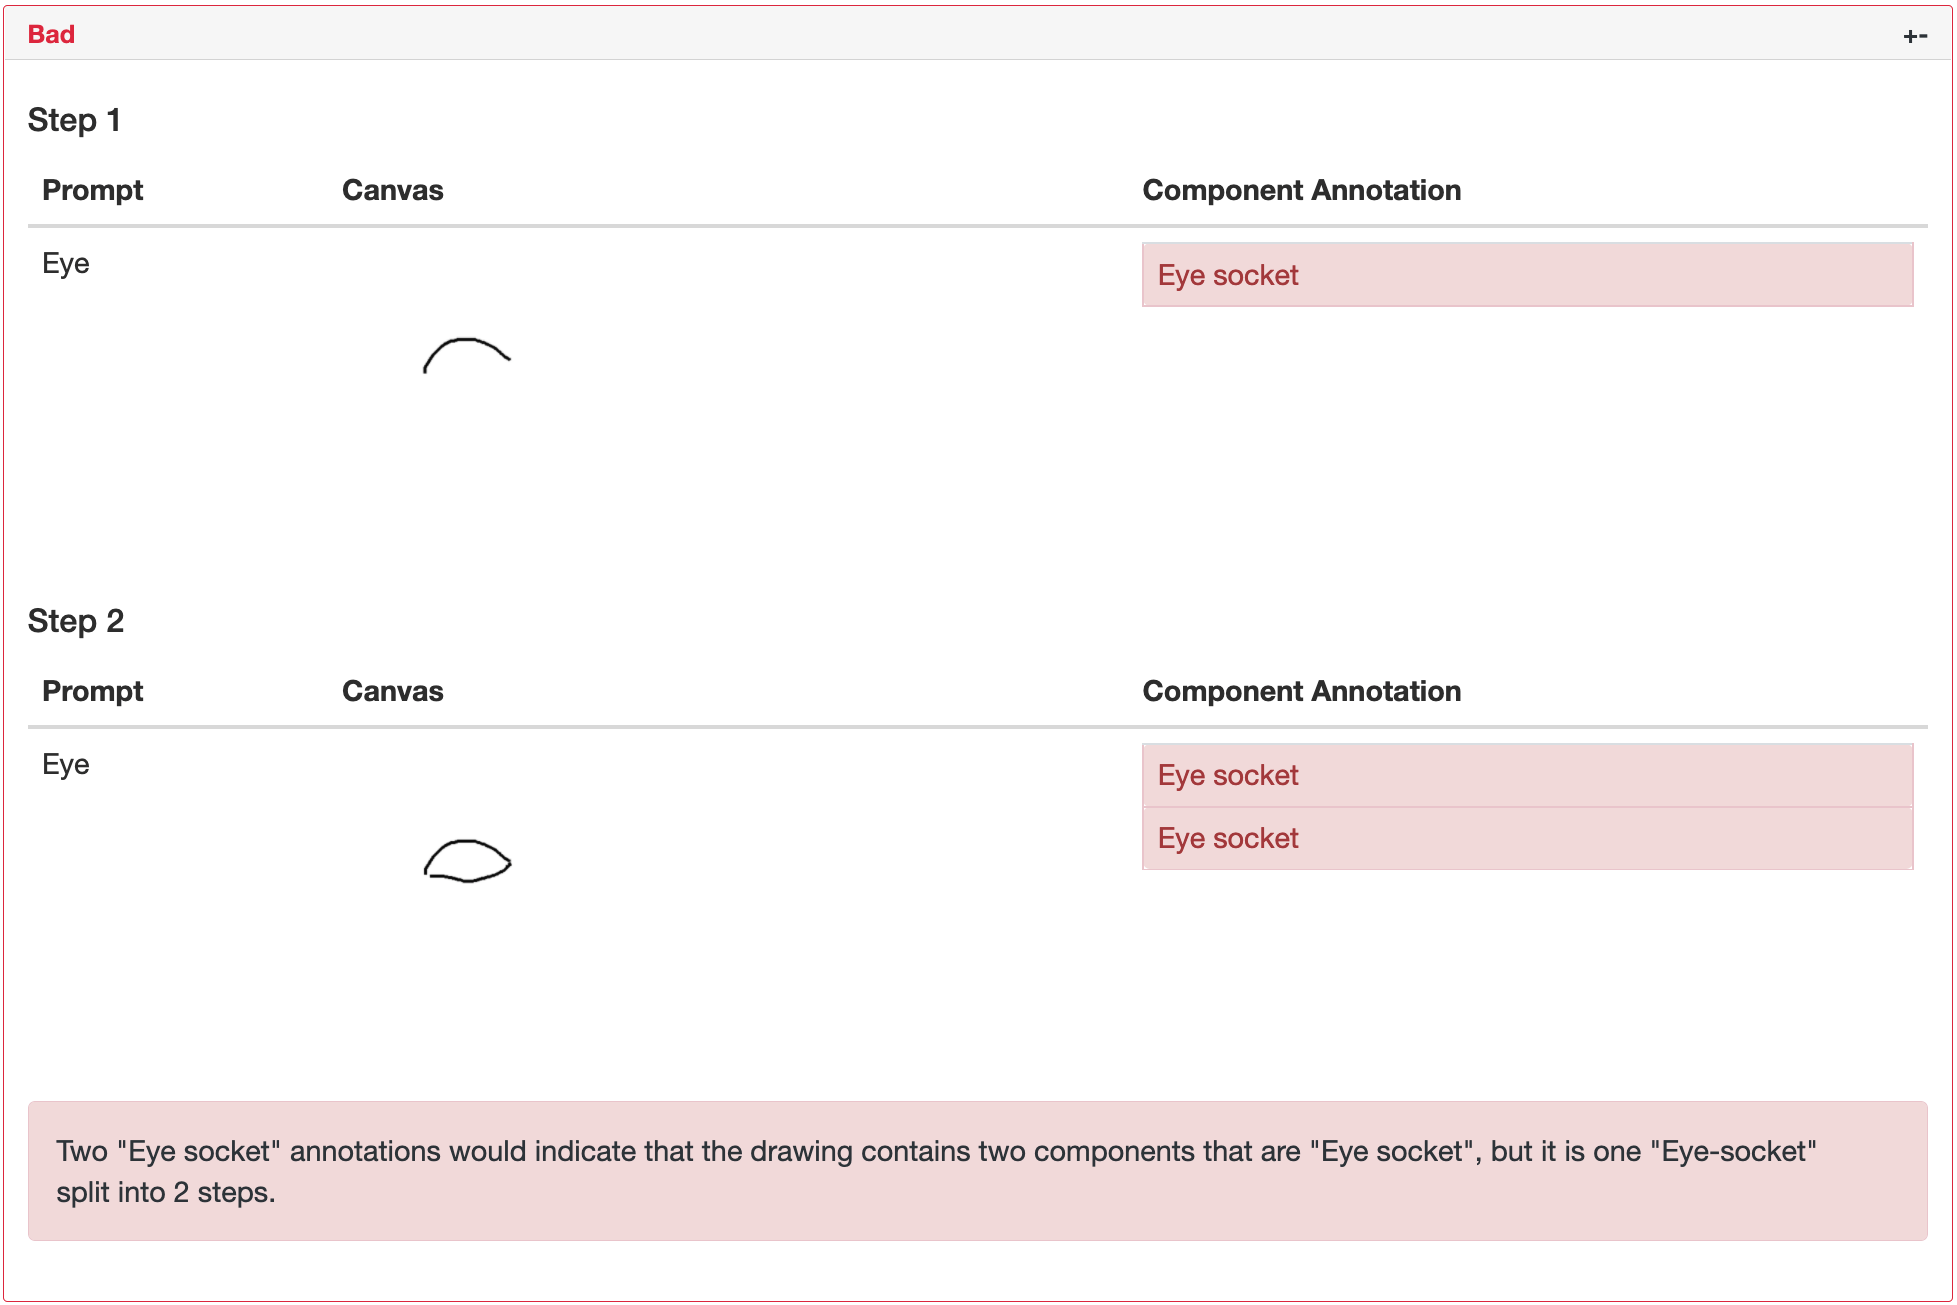
\includegraphics[width=.8\linewidth]{data_collection/v1_requirement1_bad2.png}  
    \caption{An example of misalignment: text description \textit{overflow} into multiple steps.}
    \label{v1.requirement_1.3}
\end{subfigure}
\caption{Screenshots of counterexamples used in first version of the requirements in Version 1.}
\label{v1.requirement_1}
\end{figure*}
% Figure 3x.a and 3x.b show some previous versions of the requirements. We eventually decided that  

% There is even more effort that went into defining the requirements of the task. This is really the section that we want to use to enforce all the DQ's. The final set of instructions is displayed in Figure x4.
% [Figure x4: final requirements]

% Comparing examples in requirements format:

% Methods to help understand the requirements. 
% Specifying which examples demonstrate which requirements, add next to the questions which requirement the question is testing. 

Requirements and selected examples used in the second release in lab (Item 4 is meant to enforce principal \ref{data_design_1}; the other items for \ref{data_design_2} and \ref{data_design_3}):
\begin{enumerate}
\item Draw \textit{one} item at a time and provide its corresponding annotation. For example, the text annotation says ``left eye'', but two items are drawn: a left eye and a right eye.
\item The annotation should describe its corresponding item in the drawing \textit{entirely}.
\item The annotation should name the item.
\item Desired properties of good drawings:
\begin{itemize}
    \item Contain as many items as possible, but be sure that they all contribute to illustrating the prompt. For example, draw more than just two eyes for a face.
    \item Use shapes creatively. For example, draw a triangle for the left eye, and annotate accordingly with ``triangular left eye that shows suspicion''.
\end{itemize}
\item Desired properties of good annotations:
\begin{itemize}
    \item Use descriptive languages. For example, ``a left eye that looks an arc facing downward''.
    \item Include the intention/purpose of drawing an item. Explain in the annotation reasons for drawing the item. For example, ``thumbs-up next to the face that really shows how happy the face is''.
\end{itemize}
\end{enumerate}

Requirements and selected examples used in the third release in lab (Item 1 is meant to enforce principal \ref{data_design_1}; the other items for \ref{data_design_2} and \ref{data_design_3}):
\begin{enumerate}
\item Each drawing should contain at least 2 steps.
\item Annotation of each step should include at least the name of the drawn object(s).
\item If draw multiple copies of the same object, draw each object in a separate step and give different annotations by using, for example, cardinal or ordinal numbers. (An example shown in Figure \ref{v1.requirement_3})
\item Differentiate between plural and singular forms.
\item The name of the whole should not be used for its parts. (An example shown in Figure \ref{v1.requirement_3})
\item The word "right" always refers to this side: $\Longrightarrow$
\end{enumerate}

\begin{figure*}[!htb]
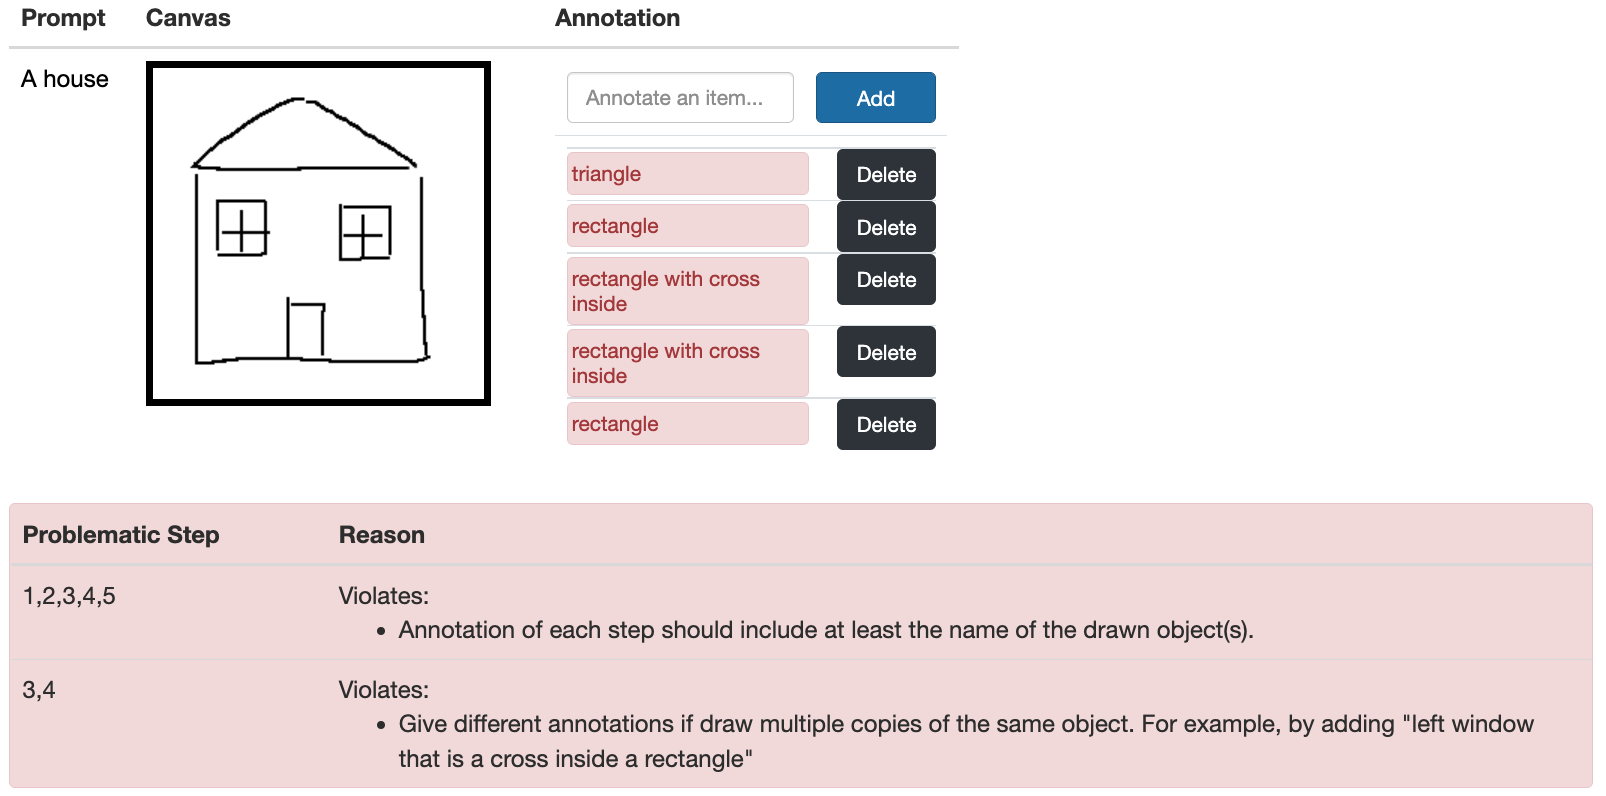
\includegraphics[width=.8\linewidth]{data_collection/v1_requirement3_bad1.png}  
\caption{Screenshots of counterexamples used in third version of the requirements in Version 1.}
\label{v1.requirement_3}
\end{figure*}

After a series of smaller changes, we eventually arived at the final version of the requirements for Version 1, as shown in Figure \ref{v1.requirement}. Most of the requirements are dedicated to ensure principle \ref{data_design_2} and \ref{data_design_3}. Requirement 1 ensures that no irrelevant sketches and trivial annotations are provided, and we resort to good faith that the annotators would provide a sketch that illustrates the given prompt. As expected, problems related to ambiguous sketches and unaligned text annotations surfaced after the deployment on AMT, eventually resulting in a complete change in format and lead to Version 2.     

\begin{figure*}[!htb]
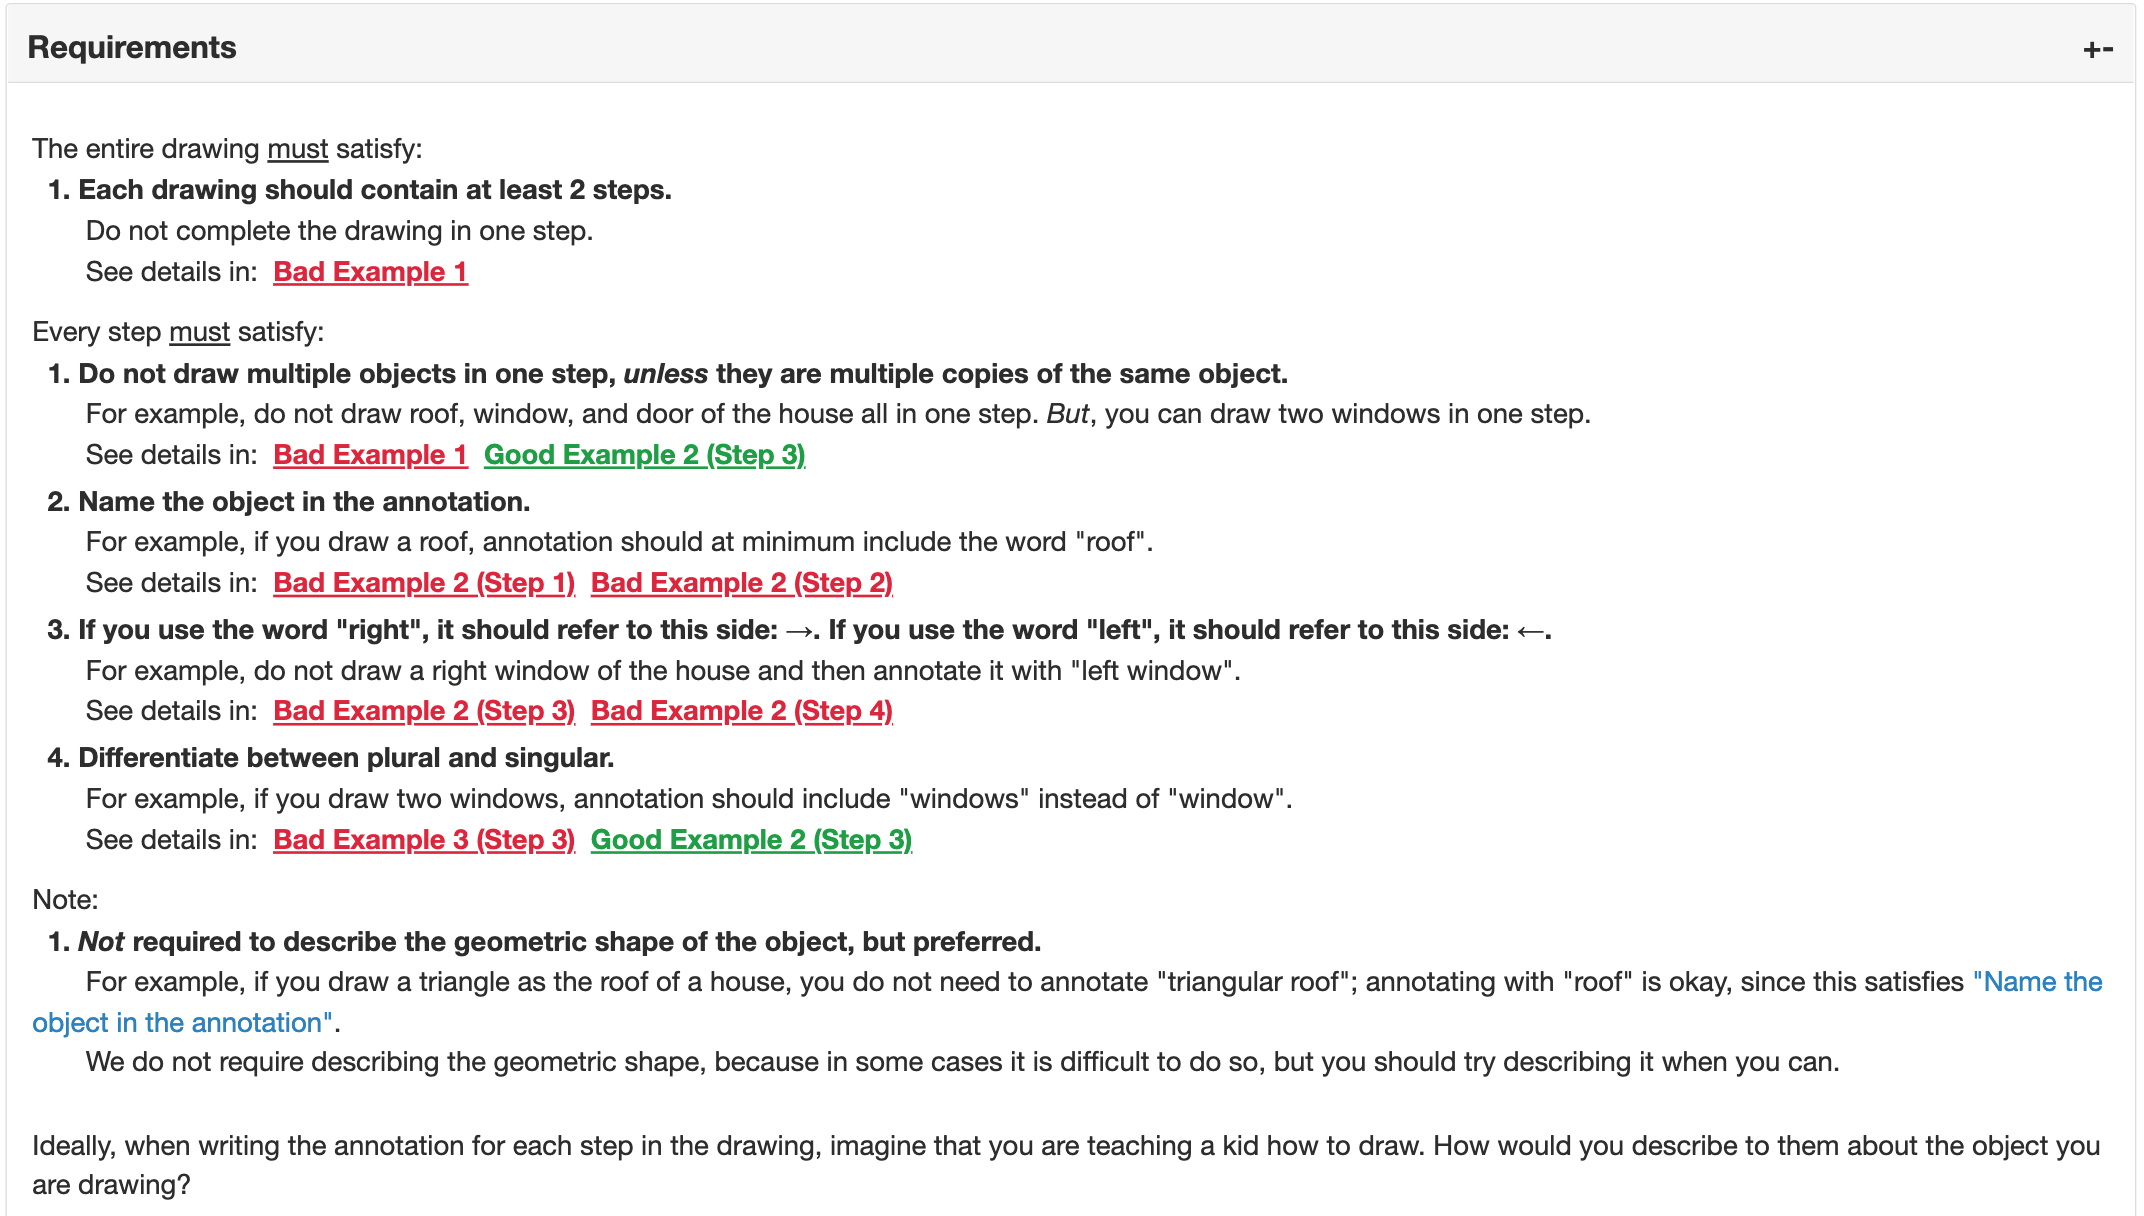
\includegraphics[width=\linewidth]{data_collection/v1_requirement.png}  
\caption{Screenshots of final version of the requirements in Version 1. The \textcolor{red}{\underline{Bad Example}} links to counter-examples of the requirements, and \textcolor{green}{\underline{Good Example}} links to good examples. When turkers click on the links, they are directed to the examples illustrating the corresponding requirement.}
\label{v1.requirement}
\end{figure*}

\begin{figure*}[!htb]
\begin{subfigure}{\textwidth}
\centering
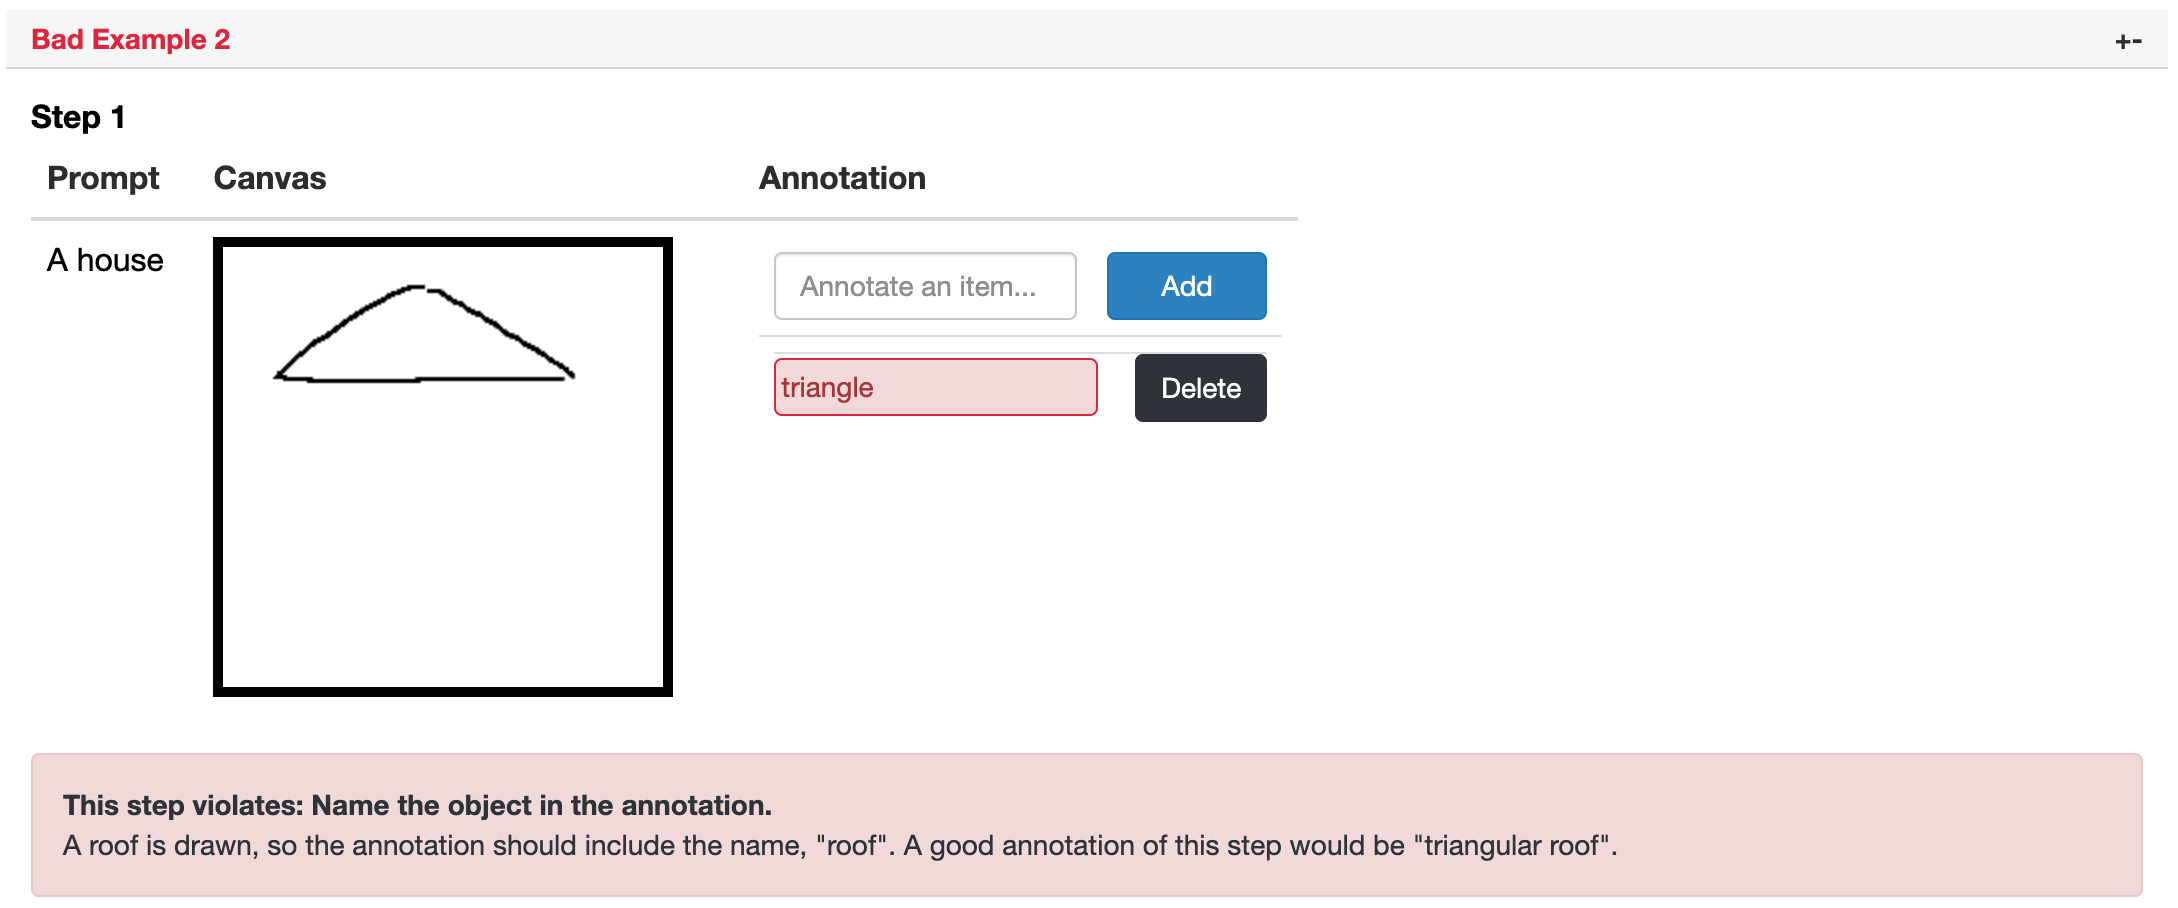
\includegraphics[width=.8\linewidth]{data_collection/v1_badeg_1.png}  
\end{subfigure}
\newline
\begin{subfigure}{\textwidth}
\centering
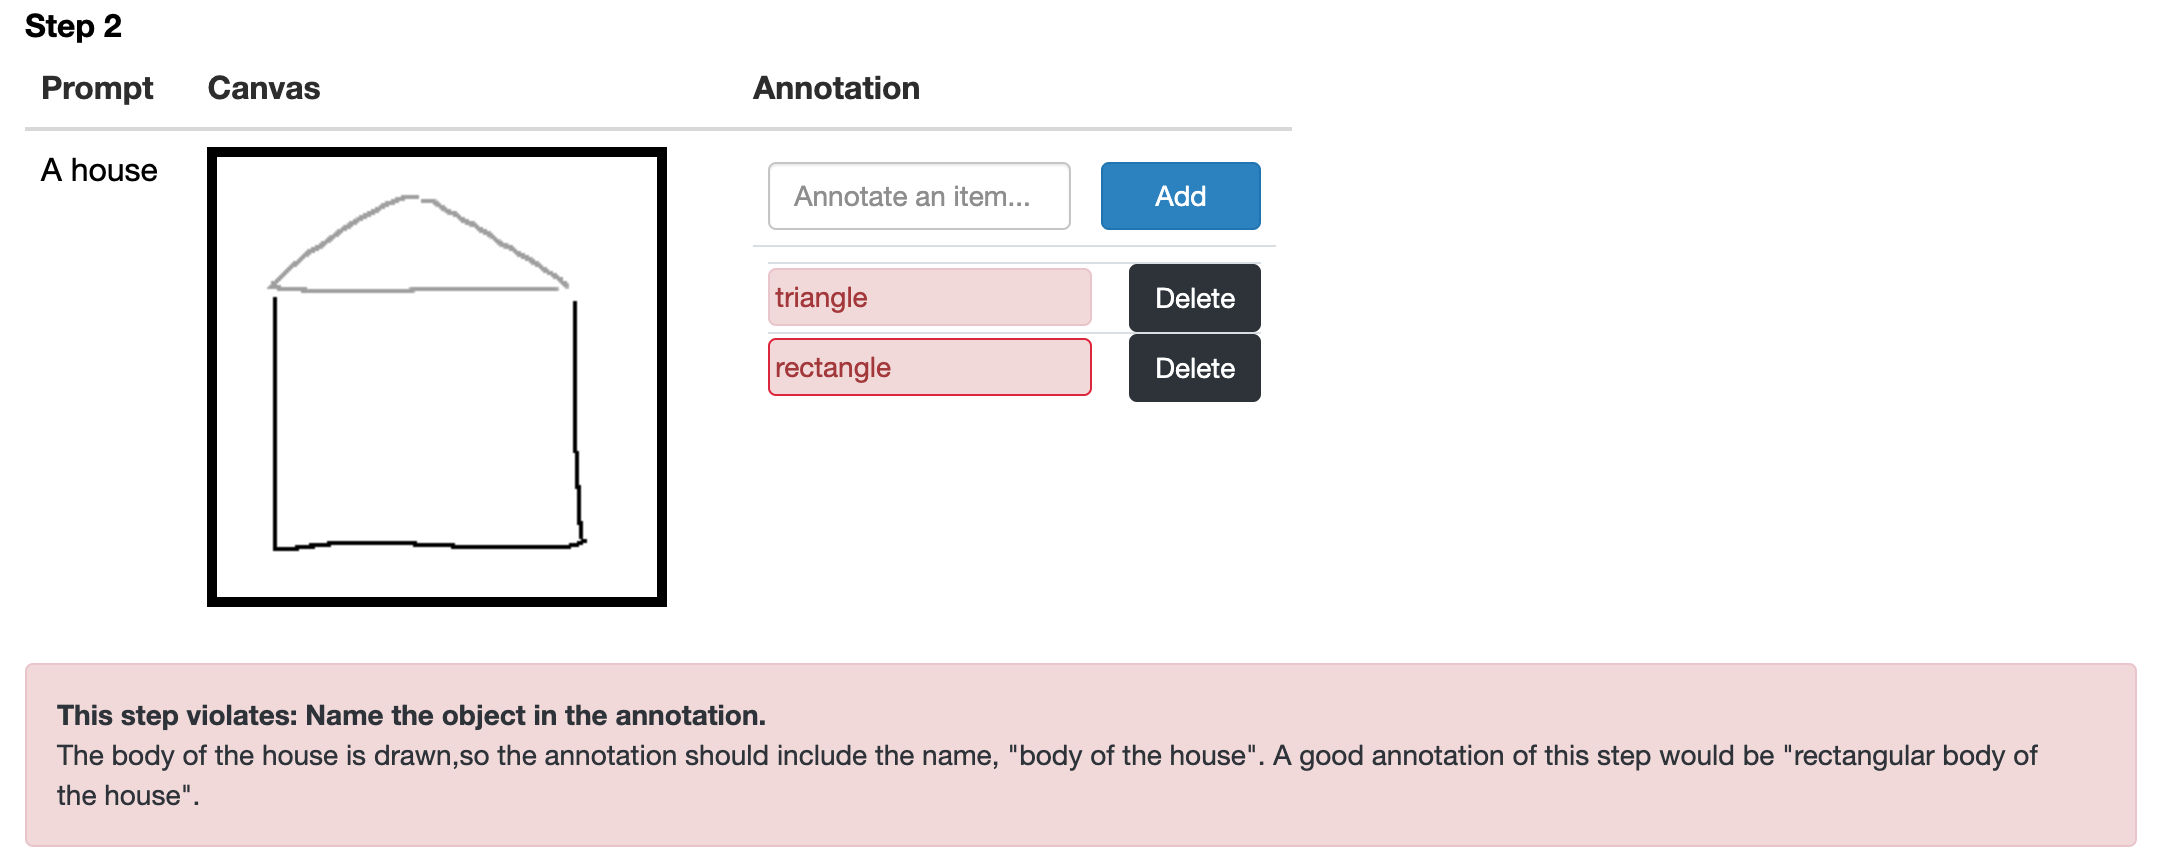
\includegraphics[width=.8\linewidth]{data_collection/v1_badeg_2.png}  
\end{subfigure}
\newline
\begin{subfigure}{\textwidth}
\centering
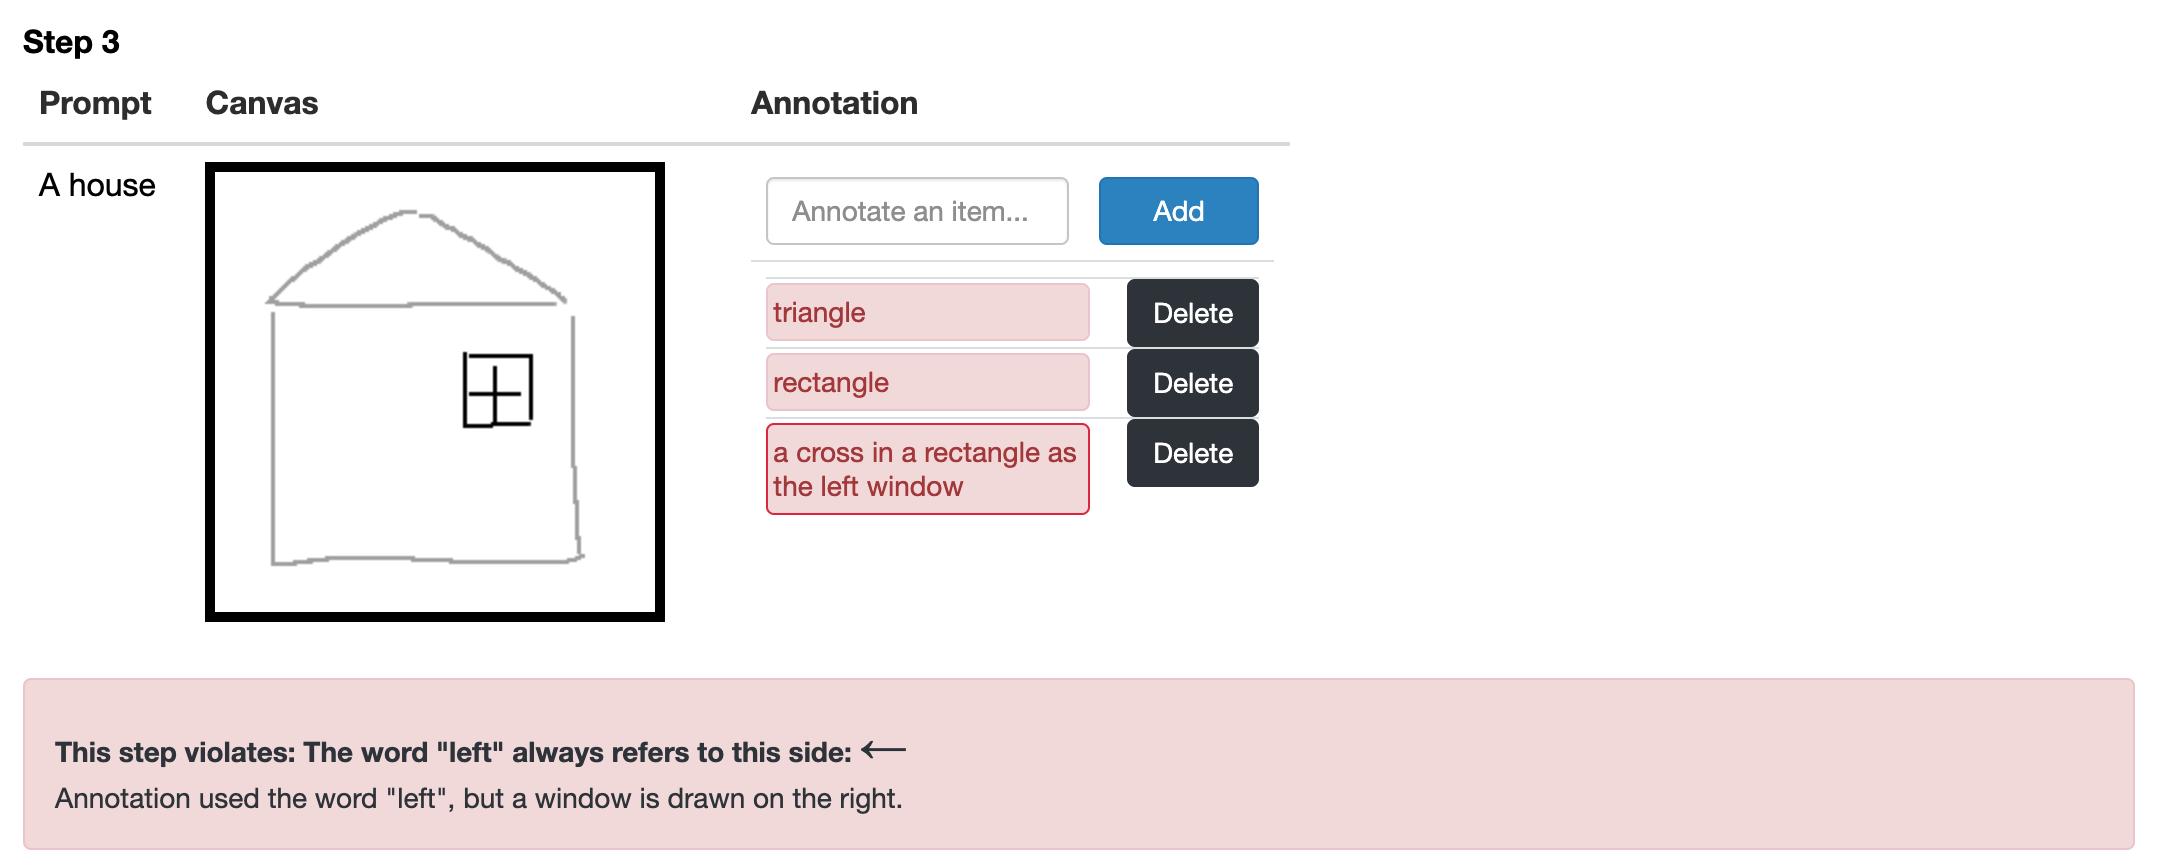
\includegraphics[width=.8\linewidth]{data_collection/v1_badeg_3.png}  
\end{subfigure}
\newline
\begin{subfigure}{\textwidth}
\centering
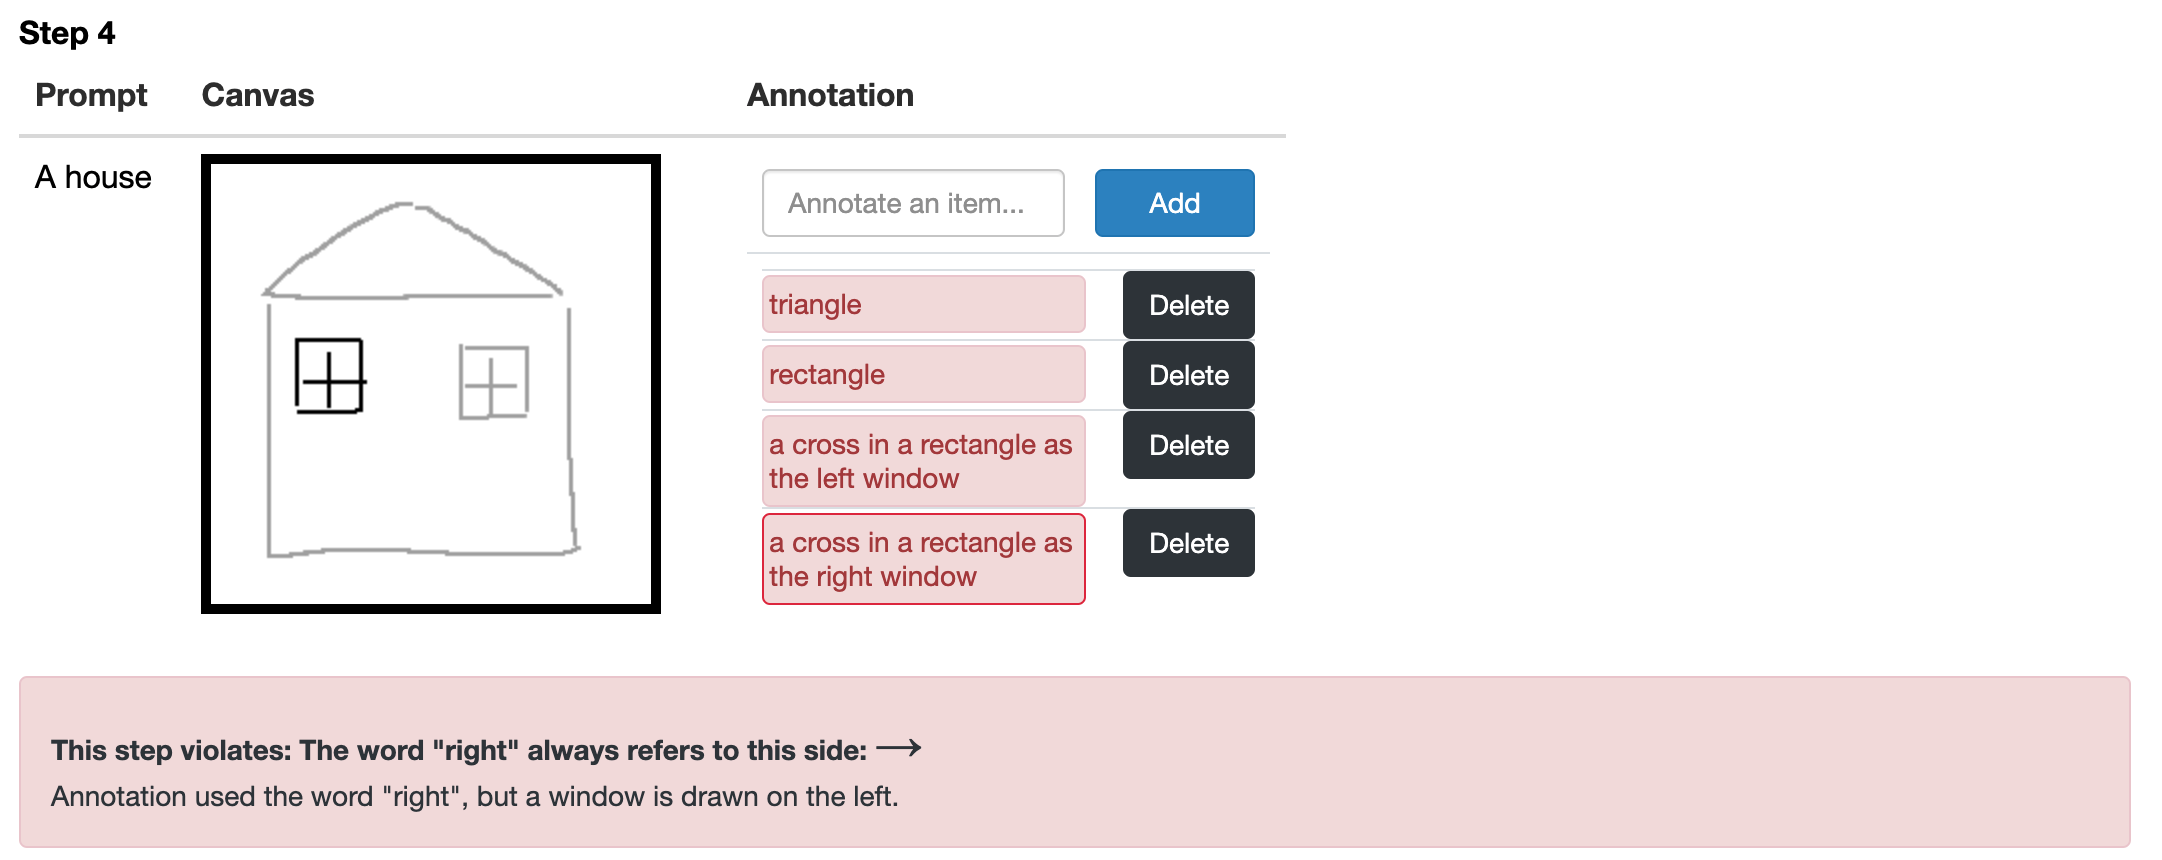
\includegraphics[width=.8\linewidth]{data_collection/v1_badeg_4.png}  
\end{subfigure}
\caption{Screenshots of an example in final version of the requirements in Version 1.}
\label{v1.badeg}
\end{figure*}

We also show \textcolor{red}{\underline{Bad Example 2}} in Figure \ref{v1.badeg} as an instance of the examples used in the final requirements. To view all the examples, refer to: \url{https://erinzhang1998.github.io/portfolio/amazon_anno}. 

\subsubsection{Qualification}

\begin{figure*}[!htb]
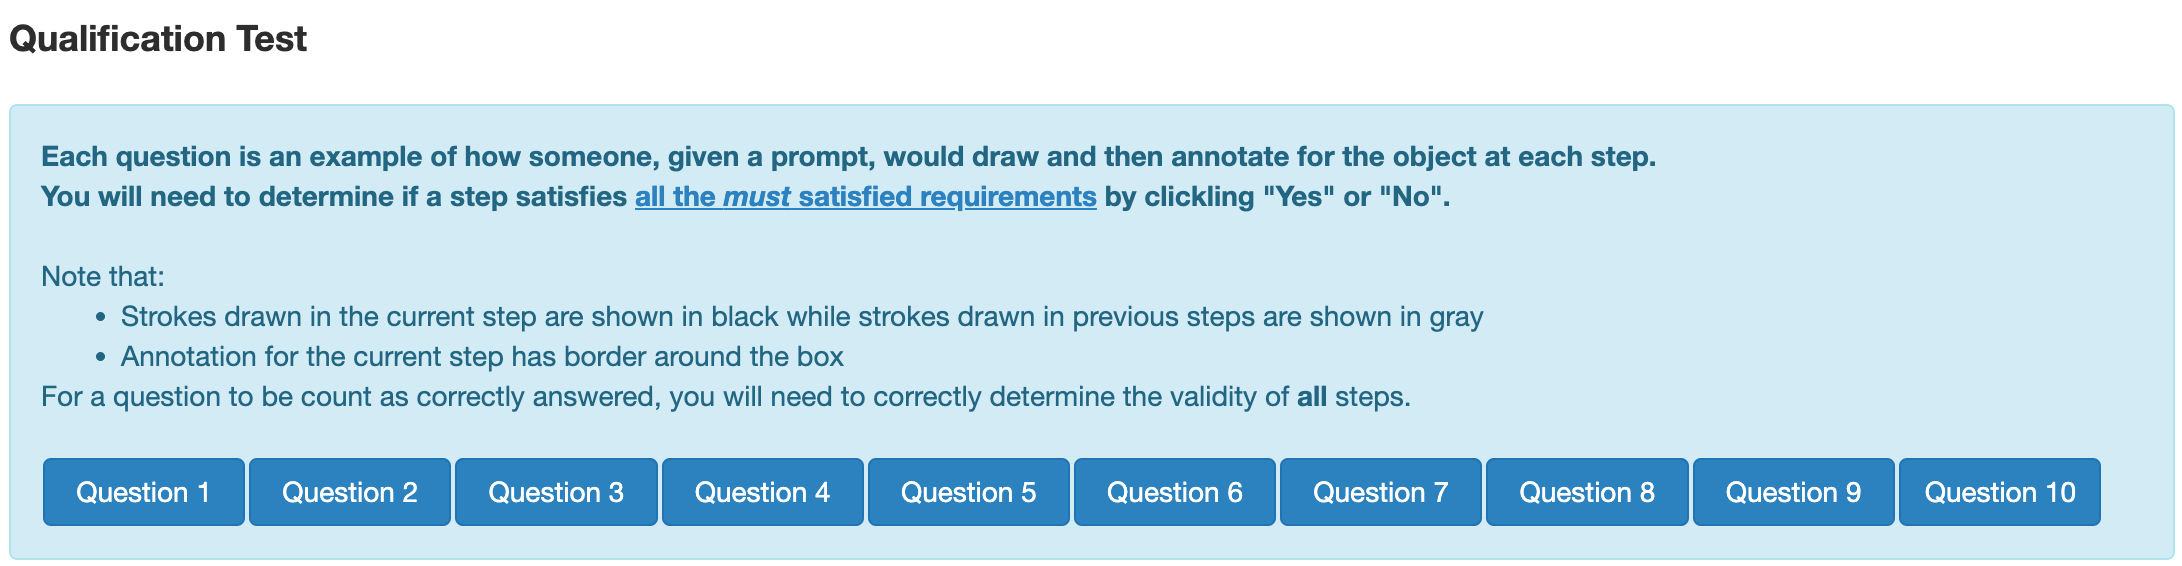
\includegraphics[width=\linewidth]{data_collection/v1_qual_header.png}  
\caption{Screenshots of the navigation bar in the qualification test of Version 1.}
\label{v1.qualification.nav}
\end{figure*}

\begin{figure*}[!htb]
\begin{subfigure}{\textwidth}
\centering
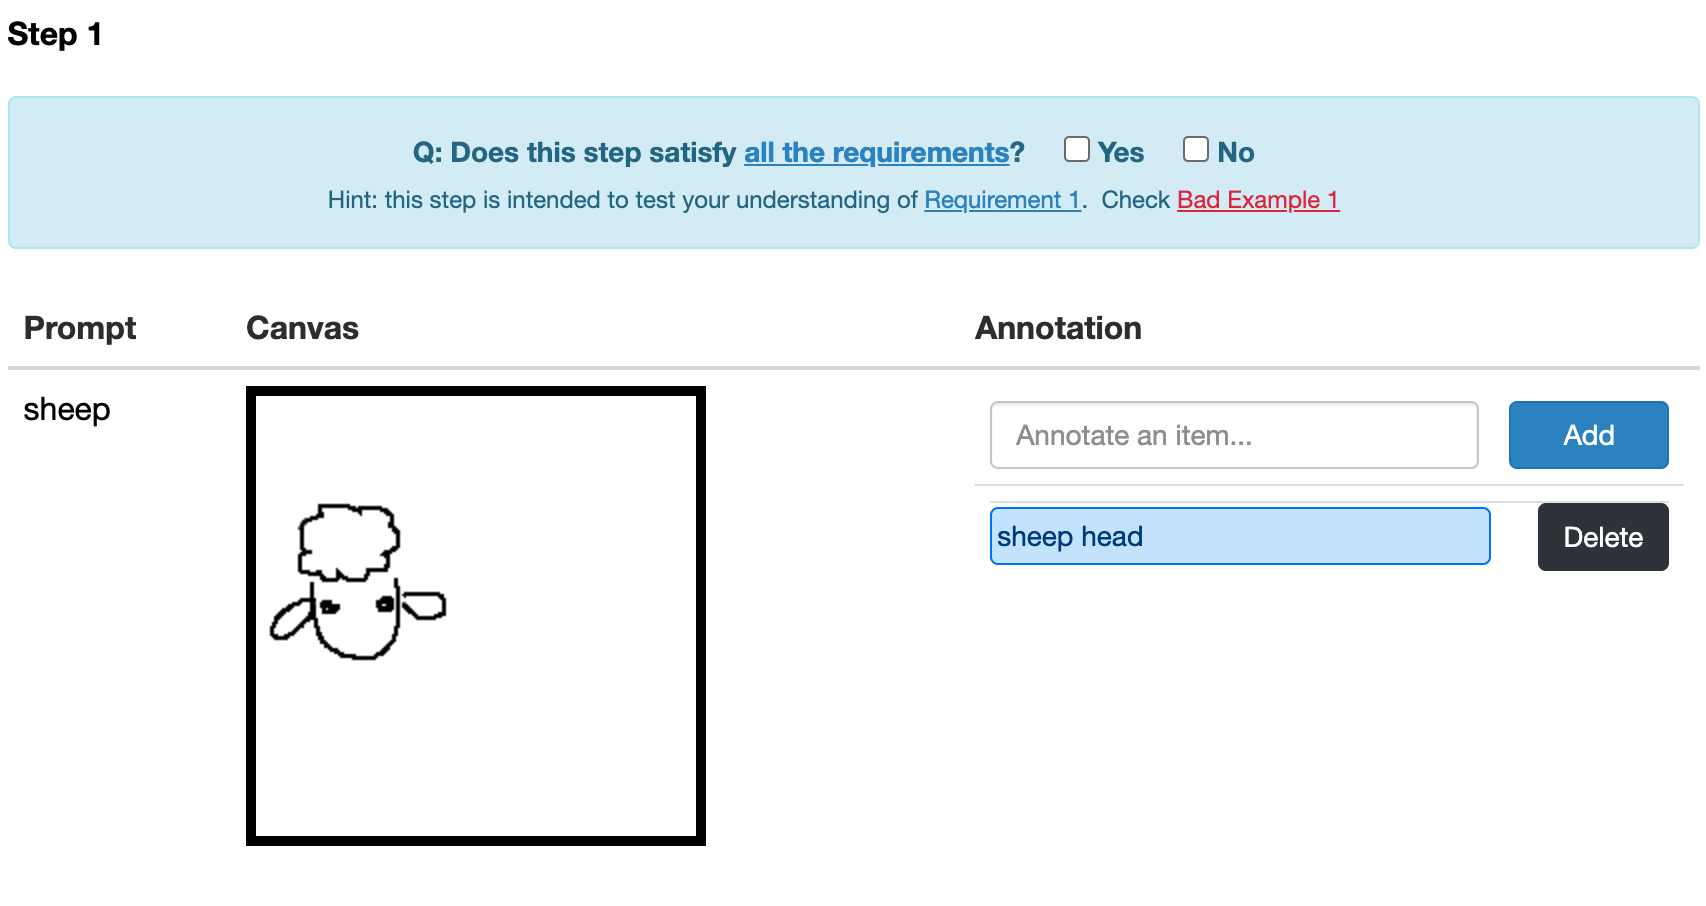
\includegraphics[width=.8\linewidth]{data_collection/v1_qual_q9_1.png}  
\end{subfigure}
\newline
\begin{subfigure}{\textwidth}
\centering
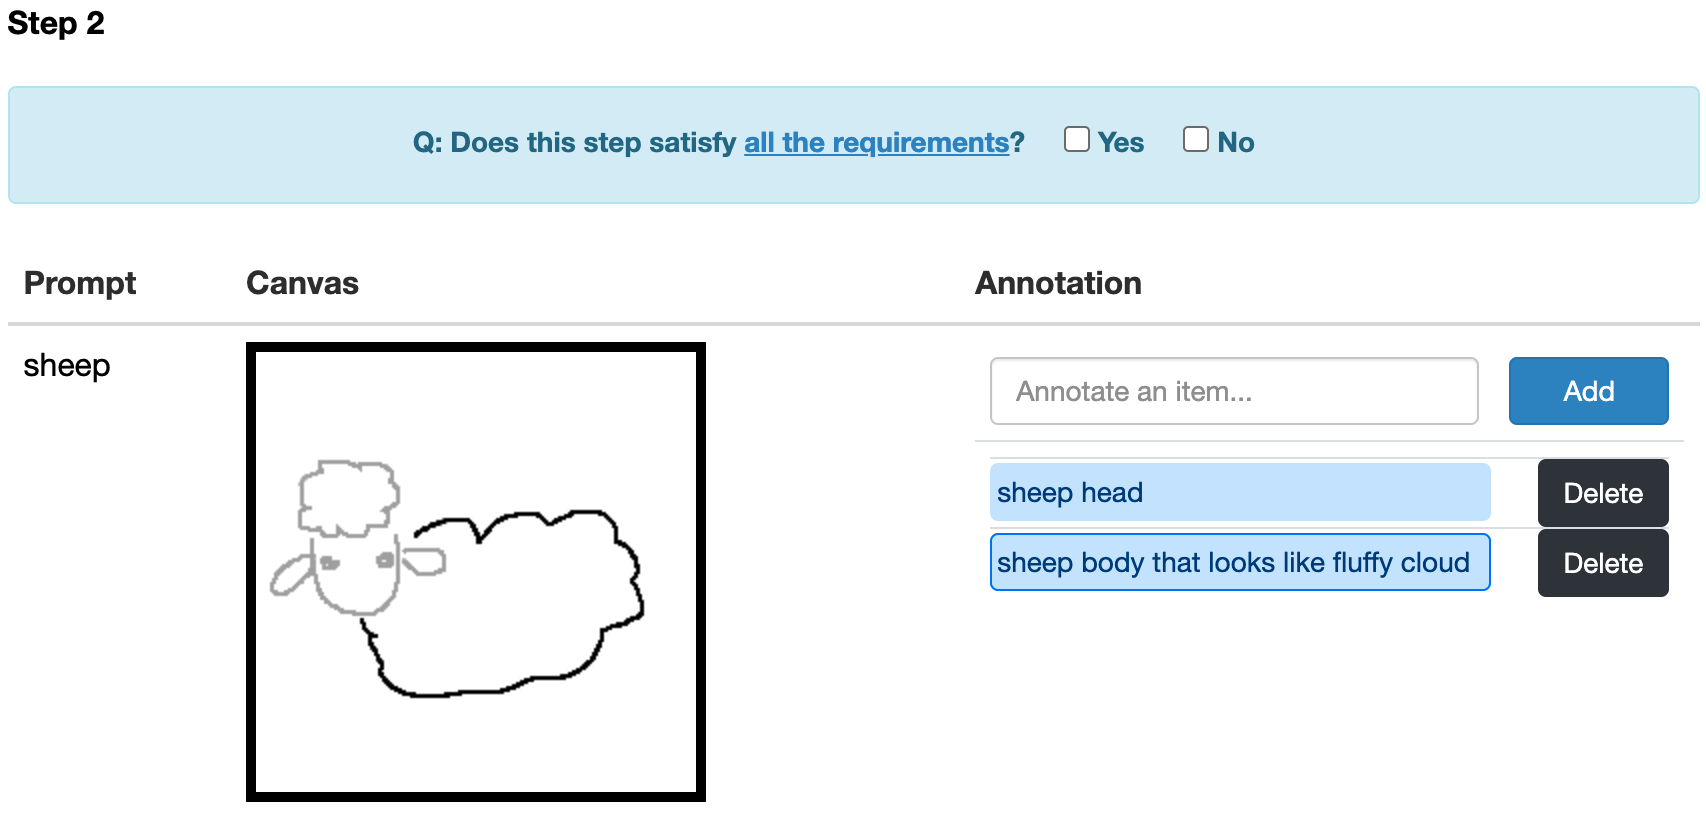
\includegraphics[width=.8\linewidth]{data_collection/v1_qual_q9_2.png}  
\end{subfigure}
\caption{Screenshots of question 9 in the qualification test of Version 1.}
\label{v1.qualification.q9}
\end{figure*}

We setup a qualification test on AMT to (1) train turkers to have better understanding of the task and (2) to select turkers who can provide annotations that satisfy all the requirements. Similar to the process of writing the requirements, we went through several rounds of testing with students in the lab to come up with a set of questions that have good correspondence with the requirements. The qualification test starts with the same instruction and requirements that will be used in the final HIT, thus allowing turkers to familiarize themselves with the requirements; moreover, this give them a chance to ask for clarifications before the final HIT. The test leads with a navigation bar (Figure \ref{v1.qualification.nav}) to make it convenient for turkers to switch between questions; originally, we displayed all questions in one page, but some people found it time-consuming to scroll from the later questions back up to the instructions, so we decided to display one question at a time. 
% We have refined the format of the qualification as we gathered feedback from people in the lab; we show a subset of the intermediate versions in Figure.
We show one question from the final qualification in Figure \ref{v1.qualification.q9}. We replicate the exact main task interface in the qualification test, and turkers need to determine whether every step of the mock annotation satisfies all the requirements; we also include hints on which requirement the question is testing for to encourage turkers to revisit the requirements and form better understanding of the task.  
To see the full test, refer to: \url{https://erinzhang1998.github.io/portfolio/amazon_qual}.

% [Figure x5: final qualification test]
%  At first, we asked the annotators to select which steps of the annotations satisfy the requirements (Figure x6.a); in order to use repetition to ensure deep understanding of the requirements, we changed to asking a yes/no question for every step, as shown in Figure x6.b.  

\subsection{Deployment Results}

% In order to determine how feasible the task is, we first deployed a version among lab members, and we obtained 55 drawings along with their annotations. All 55 drawings are shown in Figure v1.results.2. Some examples of step annotations are shown in Figure v1.results.3.  

% [Figure v1.results.2: 55 drawings from lab deployment (see jupyter notebook oct\_28\_trial\_analysis)]
% [Figure v1.results.3: 3 examples?]
To deploy our first pilot, we need to come up with a set of prompts that are in the forms of \textit{adjective}$\times$\textit{noun}. The list of adjectives includes: 
\textit{happy, sad, surprised, sleepy, lovestruck, evil};
% \textit{happy}, \textit{sad}, \textit{surprised},\textit{sleepy},\textit{lovestruck},\textit{evil}; 
the list of nouns includes: 
\textit{person, kid, cat, bear, dog, sheep, jellyfish, cup of boba, apple, burger, sun, moon, star}.
% \textit{person}, \textit{kid}, \textit{cat}, \textit{bear}, \textit{dog}, \textit{sheep}, \textit{jellyfish}, \textit{cup of boba}, \textit{apple}, \textit{burger}, \textit{sun}, \textit{moon}, \textit{star}. 
We hope to test what drawings and text descriptions annotators would provide for prompts that ask for imaginative beings not in this world, such as \textit{evil apple} or \textit{lovestruck moon}. Our first reason for doing so was that current text-to-image synthesis models, such as DALL-E and GPT-3, can produce creative artwork from abstract prompts that include novel compositions of unrelated concepts; we want to create a dataset that has the capacity to support learning models that can similarly respond to these imaginative prompts through interactive drawing. 
[!] Moreover, if we backtrack to version 0 for a second, the reason why we considered basic geometric shapes was because we are interested in how humans are able to transfer the usage of a circle to different context: a large circle could be a face, an eye, a big piece of cherry, or a moon, so transferring the same visual concept to different sketches. Also there is an aspect of transferring the same language to different context, such as in what ways the adjectives demonstrate the same concept across different object and in what ways they adapt and show different visual qualities when used on different objects.   
% The compositional nature of language allows us to put together concepts to describe both real and imaginary things. We find that DALL·E also has the ability to combine disparate ideas to synthesize objects, some of which are unlikely to exist in the real world. We explore this ability in two instances: transferring qualities from various concepts to animals, and designing products by taking inspiration from unrelated concepts.

[Figure v1.results.4: drawings from the amt pilot]

What surprised us was the amount of time turkers spent on the task. Histograms of time each annotator spent on the task is illustrated in Figure v1.results.1. Statistics of the distributions are shown in Table v1.results.1. The discrepancy might be caused by the fact that lab members with their background in computer science have an implicit understandings of what kind of quality data are needed to train ML models.   

[Figure v1.results.1: a: oct 28 lab deployment. b: dec 28 amt deployment]
[Table v1.results.1: comparing the statistics of lab vs. amt deployment]

In violation of DQ \ref{data_design_1}. Drawing does not illustrate the prompt well. The quality of the drawings are greatly influenced by how well the annotator can understand the prompts. Drawing is by its nature very subjective, so when we were examining through the sketches that we collected, we were not able to understand in what ways some sketches convey the prompts. 
[Figure v1.results.4: some examples of sketches that cannot illustrate the prompt from our perspective]

In violation of DQ \ref{data_design_2} and \ref{data_design_3}. Another problem was that annotators often fail to describe every parts they drew in one step, or the descriptions miss some parts in the step, or the description does not align well with the drawings.   
[Figure v1.results.5: some examples of mis-aligned descriptions]